%==============================================================================
%  SCE 672 Advanced Robotics (Term 261) - Assessment 2 Technical Report
%  Differential Flatness Pursuit and Motor Voltage Dynamics (RoboMaster EP Core)
%  Overleaf: upload overleaf_upload.zip (main.tex, sections/, figures/, kfupm_logo.png),
%  compile with pdfLaTeX. Figures and generated tables come from analysis/run_all.py.
%==============================================================================
\documentclass[11pt,a4paper]{article}

%------------------------------ STUDENT DETAILS -------------------------------
\newcommand{\studentName}{Ziad Aboelkhir}
\newcommand{\studentID}{g202622300}
\newcommand{\studentProgram}{Ph.D. (Direct), Systems \& Control Engineering}
\newcommand{\studentDept}{Control \& Instrumentation Engineering (CIE)}
\newcommand{\instructor}{Prof.\ Aamer Iqbal Bhatti}
\newcommand{\courseCode}{SCE 672}
\newcommand{\courseName}{Advanced Robotics}
\newcommand{\termLine}{Term 261 (Fall 2026)}
\newcommand{\submitDate}{October 26, 2026}
\newcommand{\repoURL}{https://github.com/Ziad-Behairy/advanced-robotics-project-2}
% >>> PLACEHOLDER: replace with the shared link of video/A2_demo_side_by_side.mp4 <<<
\newcommand{\videolink}{VIDEO-LINK-TBD}

%-------------------------------- PACKAGES ------------------------------------
\usepackage[a4paper,top=2.3cm,bottom=2.3cm,left=2.2cm,right=2.2cm,headheight=16pt]{geometry}
\usepackage[T1]{fontenc}
\usepackage{lmodern}
\usepackage{microtype}
\DisableLigatures[-]{encoding = T1, family = tt*}
\linespread{1.04}
\usepackage{graphicx}
\usepackage[table]{xcolor}
\usepackage{fontawesome5}
\usepackage{tabularx,booktabs,array,multirow}
\usepackage{enumitem}
\usepackage[most]{tcolorbox}
\usepackage{amsmath,amssymb,bm}
\usepackage{tikz}
\usetikzlibrary{arrows.meta,positioning,calc,fit,backgrounds,shapes.geometric,shapes.misc,decorations.pathreplacing,patterns}
\usepackage{listings}
\usepackage{caption}
\usepackage{subcaption}
\usepackage{float}
\usepackage{titlesec}
\usepackage{fancyhdr}
\usepackage[hidelinks]{hyperref}

%--------------------------------- COLOURS ------------------------------------
\definecolor{kfupm}{RGB}{12,126,64}
\definecolor{kfupmdark}{RGB}{6,84,42}
\definecolor{kfupmlight}{RGB}{233,244,237}
\definecolor{ink}{RGB}{33,37,41}
\definecolor{muted}{RGB}{105,112,120}
\definecolor{warn}{RGB}{176,96,0}
\definecolor{alert}{RGB}{190,50,45}
\definecolor{accblue}{HTML}{2A78D6}
\definecolor{accorange}{HTML}{EB6834}
\definecolor{accpurple}{HTML}{7B3FA0}
\definecolor{accgold}{HTML}{D4A017}
\definecolor{accred}{HTML}{C0392B}
\definecolor{codebg}{RGB}{246,248,247}
% mission states (same colors as every plot)
\definecolor{cSEARCHING}{HTML}{EB6834}
\definecolor{cALIGNING}{HTML}{2A78D6}
\definecolor{cCHASING}{HTML}{0B7A3E}
\definecolor{cARRIVED}{HTML}{7B3FA0}
\color{ink}

\hypersetup{
  colorlinks=true, linkcolor=kfupm, urlcolor=kfupm, citecolor=kfupm,
  pdftitle={SCE 672 Assessment 2: Differential flatness pursuit and motor voltage dynamics},
  pdfauthor={\studentName}, pdfsubject={SCE 672 Advanced Robotics, Assessment 2},
  pdfkeywords={RoboMaster EP, ROS 2 Jazzy, AprilTag, differential flatness, cubic trajectory, motor voltage}
}

%---------------------------------- LAYOUT ------------------------------------
\setlength{\parindent}{0pt}
\setlength{\parskip}{5pt}
\raggedbottom
\setlength{\intextsep}{9pt plus 2pt minus 2pt}
\setlist{itemsep=2pt,parsep=0pt,topsep=3pt,leftmargin=1.4em,labelsep=0.5em}
\setlist[itemize]{label=\textcolor{kfupm}{\scriptsize\faCaretRight}}
\setlist[enumerate]{label=\textcolor{kfupm}{\bfseries\arabic*.}}
\renewcommand{\arraystretch}{1.25}
\DeclareRobustCommand{\code}[1]{\texttt{\detokenize{#1}}}
\newcommand{\link}[2]{\href{#1}{\textcolor{kfupm}{#2}}}
\newcommand{\hd}[1]{\textcolor{white}{\bfseries #1}}      % table header cell
\newcommand{\lead}[1]{\textbf{\color{kfupmdark}#1}\enspace}  % run-in paragraph lead
% colored state badge, e.g. \stbadge{CHASING}
\newcommand{\stbadge}[1]{{\setlength{\fboxsep}{1.6pt}\colorbox{c#1!16}{\textcolor{c#1}{\scriptsize\bfseries\sffamily #1}}}}

% section style: green numbered badge + title + thin rule
\titleformat{\section}[hang]{\normalfont\LARGE\bfseries\color{kfupmdark}}
  {\tikz[baseline=(b.base)]\node[fill=kfupm,text=white,rounded corners=3pt,inner sep=4pt,
     minimum width=20pt,font=\Large\bfseries](b){\thesection};}{10pt}{}
  [\vspace{2pt}{\color{kfupm!45}\titlerule[0.8pt]}]
\titleformat{\subsection}{\normalfont\Large\bfseries\color{kfupm}}{\thesubsection}{9pt}{}
\titlespacing*{\section}{0pt}{14pt}{8pt}
\titlespacing*{\subsection}{0pt}{10pt}{4pt}
\newcommand{\isec}[2]{\section{\texorpdfstring{\textcolor{kfupm}{#1}\hspace{8pt}}{}#2}}
\newcommand{\isub}[2]{\subsection{\texorpdfstring{\textcolor{kfupm}{\normalsize #1}\hspace{6pt}}{}#2}}

% header and footer
\pagestyle{fancy}
\fancyhf{}
\renewcommand{\headrulewidth}{0.6pt}
\renewcommand{\headrule}{\hbox to\headwidth{\color{kfupm!50}\leaders\hrule height \headrulewidth\hfill}}
\fancyhead[L]{\small\color{kfupmdark}\faRobot\ \courseCode\ \courseName\ \textbullet\ Assessment 2}
\fancyhead[R]{\small\color{muted}\studentName\ \textbullet\ \studentID}
\fancyfoot[C]{\small\color{kfupm}\bfseries\thepage}
\fancyfoot[R]{\scriptsize\color{muted}KFUPM \textbullet\ CIE}

% captions
\captionsetup{font=small,labelfont={bf,color=kfupmdark},labelsep=period,skip=5pt}
\captionsetup[sub]{font=footnotesize}

% boxes
\newtcolorbox{keybox}[2][]{enhanced,colback=kfupmlight,colframe=kfupm,arc=2.5pt,boxrule=0.7pt,
  left=7pt,right=7pt,top=4pt,bottom=5pt,fonttitle=\bfseries\small,coltitle=white,
  title={#2},attach boxed title to top left={xshift=7pt,yshift=-2mm},
  boxed title style={colback=kfupm,arc=2pt,boxrule=0pt},before skip=10pt,after skip=8pt,#1}
\newtcolorbox{bluebox}[2][]{enhanced,colback=accblue!5,colframe=accblue!80,arc=2.5pt,boxrule=0.7pt,
  left=7pt,right=7pt,top=4pt,bottom=5pt,fonttitle=\bfseries\small,coltitle=white,
  title={#2},attach boxed title to top left={xshift=7pt,yshift=-2mm},
  boxed title style={colback=accblue,arc=2pt,boxrule=0pt},before skip=10pt,after skip=8pt,#1}
\newtcolorbox{purplebox}[2][]{enhanced,colback=accpurple!5,colframe=accpurple!80,arc=2.5pt,boxrule=0.7pt,
  left=7pt,right=7pt,top=4pt,bottom=5pt,fonttitle=\bfseries\small,coltitle=white,
  title={#2},attach boxed title to top left={xshift=7pt,yshift=-2mm},
  boxed title style={colback=accpurple,arc=2pt,boxrule=0pt},before skip=10pt,after skip=8pt,#1}
\newtcolorbox{notebox}[1][]{enhanced,colback=white,colframe=kfupm!55,arc=2pt,boxrule=0.5pt,
  borderline west={2.6pt}{0pt}{kfupm},left=8pt,right=7pt,top=4pt,bottom=4pt,
  before skip=8pt,after skip=8pt,#1}
\newtcolorbox{warnbox}[1][]{enhanced,colback=warn!6,colframe=warn!70,arc=2pt,boxrule=0.5pt,
  borderline west={2.6pt}{0pt}{warn},left=8pt,right=7pt,top=4pt,bottom=4pt,
  before skip=8pt,after skip=8pt,#1}
\newcommand{\stat}[4][kfupm]{%
  \begin{tcolorbox}[enhanced,width=0.235\linewidth,nobeforeafter,colback=white,colframe=#1!60,
    borderline north={2.5pt}{0pt}{#1},arc=3pt,boxrule=0.6pt,halign=center,valign=center,height=2.4cm,left=2pt,right=2pt]
  {\color{#1}\Large #2}\\[3pt]{\color{kfupmdark}\Large\bfseries #3}\\[2pt]{\footnotesize\color{muted}#4}
  \end{tcolorbox}}

% code listings
\lstdefinestyle{sh}{language=bash,basicstyle=\ttfamily\footnotesize,backgroundcolor=\color{codebg},
  frame=leftline,framerule=2.6pt,rulecolor=\color{kfupm},xleftmargin=9pt,framexleftmargin=7pt,
  keywordstyle=\color{kfupmdark}\bfseries,commentstyle=\color{muted}\itshape,stringstyle=\color{warn},
  showstringspaces=false,columns=fullflexible,keepspaces=true,breaklines=true,upquote=true,
  aboveskip=8pt,belowskip=6pt}
\lstdefinestyle{py}{language=Python,basicstyle=\ttfamily\footnotesize,backgroundcolor=\color{codebg},
  frame=leftline,framerule=2.6pt,rulecolor=\color{accblue},xleftmargin=9pt,framexleftmargin=7pt,
  keywordstyle=\color{accblue}\bfseries,commentstyle=\color{muted}\itshape,stringstyle=\color{warn},
  showstringspaces=false,columns=fullflexible,keepspaces=true,breaklines=true,upquote=true,
  numbers=left,numberstyle=\tiny\color{muted},numbersep=6pt,aboveskip=8pt,belowskip=6pt}

% tikz styles
\tikzset{
  blk/.style={draw=kfupm,fill=kfupmlight,rounded corners=3pt,align=center,inner sep=5pt,
              font=\small,text width=#1},
  blk/.default=4cm,
  grp/.style={draw=kfupmdark,thick,rounded corners=6pt,inner sep=9pt},
  arr/.style={-{Latex[length=2.4mm]},thick,color=kfupmdark},
  biarr/.style={{Latex[length=2.4mm]}-{Latex[length=2.4mm]},thick},
  topic/.style={draw=muted,fill=white,rounded corners=1pt,font=\footnotesize\ttfamily,inner sep=3pt},
  rosnode/.style={draw=kfupm,fill=kfupmlight,ellipse,font=\footnotesize\ttfamily,inner sep=1.5pt},
  lbl/.style={font=\scriptsize,color=muted,align=center},
  stnode/.style={draw=c#1,fill=c#1!10,line width=1.1pt,rounded corners=6pt,align=center,
                 inner sep=5pt,text width=3.5cm,font=\small},
  tr/.style={-{Latex[length=2.6mm]},thick,color=ink},
  trl/.style={font=\scriptsize,align=center,fill=white,inner sep=1.5pt}
}

%==============================================================================
\begin{document}

%================================= COVER ======================================
\begin{titlepage}
\newgeometry{top=0cm,bottom=0cm,left=0cm,right=0cm}
\thispagestyle{empty}
\begin{tikzpicture}[remember picture,overlay]
  \fill[kfupm] (current page.north west) rectangle ([yshift=-6.3cm]current page.north east);
  \fill[kfupmdark] ([yshift=-6.3cm]current page.north west) rectangle ([yshift=-6.55cm]current page.north east);
  % thin colored strip with the four mission states
  \foreach \col [count=\i from 0] in {cSEARCHING,cALIGNING,cCHASING,cARRIVED}{
    \fill[fill=\col] ([xshift=\i*5.25cm,yshift=-6.55cm]current page.north west) rectangle
              ([xshift=\i*5.25cm+5.25cm,yshift=-6.75cm]current page.north west);}
  \fill[kfupm] (current page.south west) rectangle ([yshift=1.3cm]current page.south east);
  \node[fill=white,circle,inner sep=10pt,draw=kfupmdark,line width=2pt] at ([yshift=-6.4cm]current page.north)
       {
\includegraphics[width=3.9cm]{kfupm_logo.png}};
  \node[text=white,align=center,font=\Large\bfseries] at ([yshift=-1.55cm]current page.north)
       {King Fahd University of Petroleum \& Minerals};
  \node[text=white,align=center,font=\large] at ([yshift=-2.35cm]current page.north)
       {College of Engineering and Physics \textbullet\ \studentDept};
  \node[text=white,align=center,font=\normalsize] at ([yshift=0.65cm]current page.south)
       {\faUniversity\ Dhahran, Saudi Arabia \quad\textbullet\quad \submitDate};
\end{tikzpicture}
\vspace*{10.2cm}
\begin{center}
  {\color{kfupm}\large\bfseries \courseCode\ \textbullet\ \courseName\ \textbullet\ \termLine\par}
  \vspace{0.45cm}
  {\color{kfupmdark}\fontsize{26}{31}\selectfont\bfseries Assessment 2 Technical Report\par}
  \vspace{0.35cm}
  {\Large Differential Flatness Pursuit and\\[3pt] Motor Voltage Dynamics\par}
  \vspace{0.3cm}
  {\color{muted}\large AprilTag search, in-place centering, cubic flat-output pursuit and a 20\,cm halt\\
   on the DJI RoboMaster EP Core with ROS 2 Jazzy\par}
  \vspace{0.8cm}
  \begin{minipage}{16.4cm}
  \stat[kfupm]{\faBullseye}{20\,cm}{standoff, tape measured}\hfill
  \stat[accblue]{\faTachometerAlt}{0.137\,m/s}{peak speed ($v_{max}$ 0.16)}\hfill
  \stat[accpurple]{\faBolt}{0.000\,V}{all motors after ARRIVED}\hfill
  \stat[accorange]{\faVial}{36 / 36}{offline tests passed}
  \end{minipage}
  \vspace{0.8cm}

  \begin{tcolorbox}[center,width=14.2cm,colback=kfupmlight,colframe=kfupm,arc=3pt,boxrule=0.8pt,left=10pt,right=10pt]
  \large
  \begin{tabular}{@{}c@{\hspace{9pt}}l@{\hspace{12pt}}l@{}}
   \textcolor{kfupm}{\faUserGraduate}      & Student     & \textbf{\studentName}\\
   \textcolor{kfupm}{\faIdCard}            & Student ID  & \studentID\\
   \textcolor{kfupm}{\faGraduationCap}     & Program     & \studentProgram\\
   \textcolor{kfupm}{\faChalkboardTeacher} & Instructor  & \instructor\\
   \textcolor{kfupm}{\faRobot}             & Platform    & RoboMaster EP Core, ROS 2 Jazzy, Ubuntu 24.04\\
   \textcolor{kfupm}{\faCalendarCheck}     & Submitted   & \submitDate
  \end{tabular}
  \end{tcolorbox}
\end{center}
\restoregeometry
\end{titlepage}

%============================ CONTENTS & MAP =================================
\setcounter{page}{2}
{\hypersetup{linkcolor=ink}\setcounter{tocdepth}{2}\tableofcontents}
\clearpage

\begin{keybox}{\faClipboardCheck\ \ Deliverables map}
\small
\begin{tabularx}{\linewidth}{@{}l>{\raggedright\arraybackslash}X>{\raggedright\arraybackslash}p{4.4cm}@{}}
\textbf{Item} & \textbf{Content} & \textbf{Location}\\\midrule
D1 Report & flat inversion (1), boundary matrix (2) and its solver, horizon scaling (3), Table~\ref{tab:table1}
  with the measured voltages, $v(t)$ and $V_1(t)$ plot (Figure~\ref{fig:vV1}) & this PDF\\
D2 Code & ROS 2 package \code{rm_flatness_nav}: \code{tag_detector}, \code{flatness_planner}, FSM, flatness and
  voltage modules, 36 offline tests, launch file, \code{config/robot.yaml} & \link{\repoURL}{\faGithub\ private repository},
  \code{ros2/rm_flatness_nav/}\\
D2 Data & \code{motor_voltage_log.csv} of the final run (1\,s rows) plus the 20\,Hz log, all runs, calibration, raw
  driver and detector logs & repository root and \code{data/}\\
D3 Video & phone view and robot view side by side, 23.8\,s: (a) sweep while T3 is hidden, (b) centering on T3,
  (c) cruise and stop at 20\,cm & \link{\videolink}{\faVideo\ demo video} (23.8\,s)\\
\end{tabularx}
\end{keybox}

\begin{notebox}
\small\textbf{\color{kfupmdark}\faInfoCircle\ How the numbers were produced}
\begin{itemize}
  \item Every figure, table row and statistic comes from the scripts in \code{analysis/}, run on the raw files in
        \code{data/}; \code{python3 analysis/run_all.py} regenerates them and writes \code{analysis/results/summary.md}.
  \item Table~\ref{tab:table1} and the run table are generated from the CSV files as text, so the values are copied
        verbatim, without rounding or editing.
  \item Hand measurements (tape standoff after each stop, tag size, range calibration distances) were taken by the
        student and written into the \code{notes.md} of each run and \code{data/calibration/tag_range.csv};
        observations read from the terminal during the session (TF readings, arm positions, Wi-Fi events, the 1.80\,m
        probe, the drive direction test) are recorded verbatim in \code{notes/lab_log.md}.
  \item Video stills are frames of the submitted demo video; robot photos are in \code{notes/photos/}.
\end{itemize}
\end{notebox}

%============================== 1. OVERVIEW ===================================
\isec{\faProjectDiagram}{System Overview}

The mission: the robot starts with the target tag T3 out of view, sweeps in place until it sees it, turns in place
until T3 is centered, follows a cubic flat-output trajectory toward it and brakes 20\,cm before it, while logging the
four motor armature voltages. Figure~\ref{fig:arena} shows the arena used for the final run.

\begin{figure}[H]
\centering
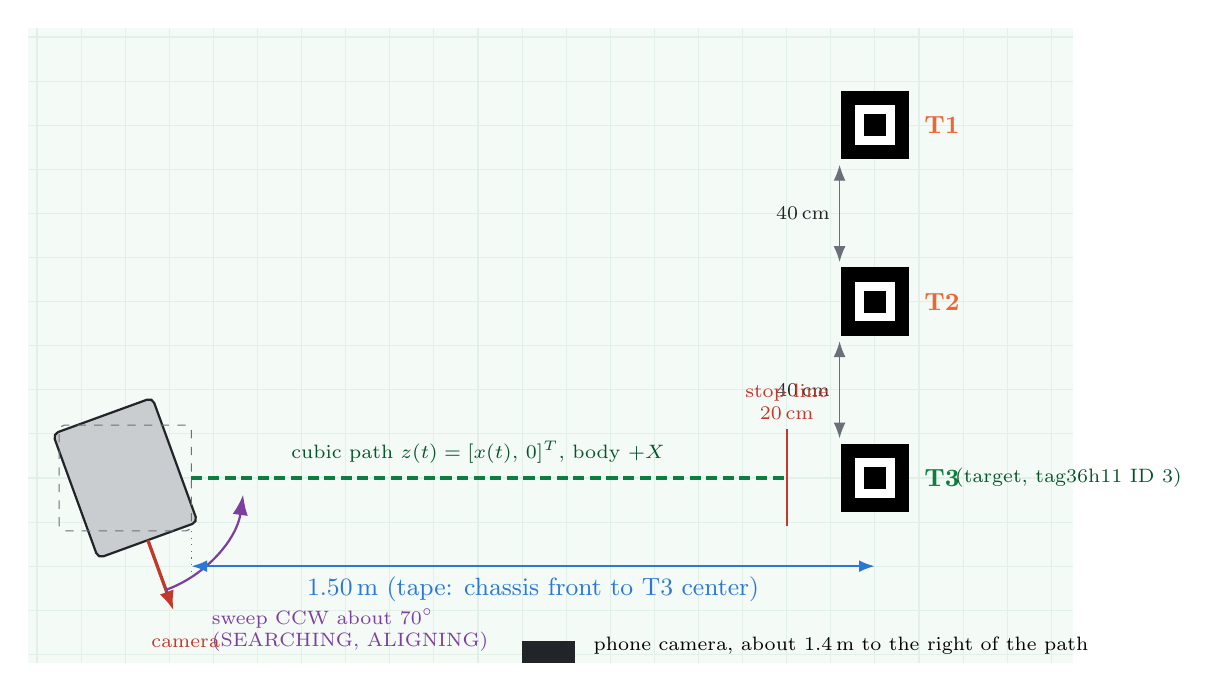
\begin{tikzpicture}[x=5.6cm,y=5.6cm,font=\small]
  % floor grid
  \fill[kfupmlight!50] (-0.42,-0.42) rectangle (1.95,1.02);
  \draw[kfupm!12,step=0.1] (-0.42,-0.42) grid (1.95,1.02);
  % tags (155 mm)
  \foreach \y/\tn/\tc in {0/T3/kfupm,0.40/T2/accorange,0.80/T1/accorange}{
    \fill[black] (1.5-0.0775,\y-0.0775) rectangle (1.5+0.0775,\y+0.0775);
    \fill[white] (1.5-0.045,\y-0.045) rectangle (1.5+0.045,\y+0.045);
    \fill[black] (1.5-0.025,\y-0.025) rectangle (1.5+0.025,\y+0.025);
    \node[font=\small\bfseries,text=\tc,right] at (1.59,\y) {\tn};}
  \node[font=\scriptsize,text=kfupmdark,right] at (1.66,0) {(target, tag36h11 ID 3)};
  \draw[{Latex[length=2mm]}-{Latex[length=2mm]},muted] (1.42,0.09) -- node[left,font=\scriptsize,text=ink]{40\,cm} (1.42,0.31);
  \draw[{Latex[length=2mm]}-{Latex[length=2mm]},muted] (1.42,0.49) -- node[left,font=\scriptsize,text=ink]{40\,cm} (1.42,0.71);
  % robot start (rotated 70 deg clockwise)
  \begin{scope}[shift={(-0.2,0)},rotate=-70]
    \draw[ink,thick,fill=muted!35,rounded corners=2pt] (-0.15,-0.12) rectangle (0.15,0.12);
    \draw[-{Latex[length=2.5mm]},very thick,accred] (0.15,0) -- (0.32,0);
    \node[font=\scriptsize,text=accred] at (0.40,0) {camera};
  \end{scope}
  \draw[dashed,muted,rounded corners=2pt] (-0.35,-0.12) rectangle (-0.05,0.12);
  \draw[-{Latex[length=2.6mm]},thick,accpurple] (-0.2,0)++(-70:0.27) arc (-70:-8:0.27);
  \node[font=\scriptsize,text=accpurple,align=left] at (0.31,-0.345) {sweep CCW about $70^\circ$\\(SEARCHING, ALIGNING)};
  % chassis front and tape distance
  \draw[{Latex[length=2mm]}-{Latex[length=2mm]},accblue,thick] (-0.05,-0.20) -- node[below,font=\small,text=accblue]{1.50\,m (tape: chassis front to T3 center)} (1.5,-0.20);
  \draw[dotted,accblue] (-0.05,-0.12) -- (-0.05,-0.22);
  % planned path and standoff
  \draw[kfupm,very thick,dash pattern=on 4pt off 2pt] (-0.05,0) -- (1.30,0);
  \node[font=\scriptsize,text=kfupmdark,above] at (0.60,0.01) {cubic path $z(t)=[x(t),\,0]^T$, body $+X$};
  \draw[accred,thick] (1.30,-0.11) -- (1.30,0.11);
  \node[font=\scriptsize,text=accred,above,align=center] at (1.30,0.11) {stop line\\20\,cm};
  % phone
  \fill[ink] (0.70,-0.42) rectangle (0.82,-0.37);
  \node[font=\scriptsize,right,align=left] at (0.84,-0.38) {phone camera, about 1.4\,m to the right of the path};
\end{tikzpicture}
\caption{Arena of the final run \code{20261026_015001} (top view, redrawn from \code{notes/final_run_setup.png}).
The robot starts turned about $70^\circ$ clockwise, so T3 is outside the camera view and the run begins in SEARCHING.
T1 and T2 are distractor tags; only ID 3 is accepted.}
\label{fig:arena}
\end{figure}

\isub{\faSitemap}{Software architecture}
The package \code{rm_flatness_nav} adds two ROS 2 nodes on top of the \code{robomaster_ros} driver \cite{rmros}
(Figure~\ref{fig:arch}). The control logic lives in plain Python modules without ROS imports, so the same code runs
in the offline tests and on the robot.
\begin{itemize}
  \item \textbf{\code{tag_detector}:} AprilTag detection \cite{olson,wang} (\code{pupil-apriltags} \cite{pupil}, family \code{tag36h11}) on the newest
        camera frame, camera pose from the floor tag, ground range $d$ and bearing $\theta$ of T3.
  \item \textbf{\code{flatness_planner}:} 20\,Hz control loop: arm guard, mission state machine (\code{mission.py}),
        flat-output plan (\code{flatness.py}), wheel rates and voltages (\code{voltage.py}), CSV and terminal logging.
\end{itemize}

\begin{figure}[H]
\centering
\begin{tikzpicture}[node distance=4mm]
  % host side
  \node[blk=4.3cm,align=left] (det) {\faCamera\ \textbf{\code{tag_detector}}\\[1pt]\footnotesize
     newest frame only, 15\,Hz timer\\ pupil-apriltags, ID 3, 155\,mm\\ $d$, $\theta$ in a level camera frame\\
     image watchdog (re-subscribe)};
  \node[blk=4.3cm,align=left,below=6mm of det] (pl) {\faCogs\ \textbf{\code{flatness_planner}} (20\,Hz)\\[1pt]\footnotesize
     arm guard (saved pose $\pm$6\,mm)\\ FSM \code{mission.py}\\ cubic plan \code{flatness.py}\\
     eq.~(4), (5) \code{voltage.py}};
  \node[blk=4.3cm,fill=white,below=6mm of pl,align=left] (csv) {\faFileCsv\ \code{motor_voltage_log.csv} (1\,s)\\
     \faFileCsv\ \code{motor_voltage_full.csv} (20\,Hz)\\ \faTerminal\ live table in the terminal};
  \begin{scope}[on background layer]
  \node[grp,fit=(det)(pl)(csv),label={[font=\small\bfseries,text=kfupmdark]above:\faLaptop\ Laptop, ROS 2 Jazzy}] (host) {};
  \end{scope}
  % driver
  \node[blk=3.7cm,right=1.3cm of pl,align=left] (drv) {\faPlug\ \textbf{\code{robomaster_ros}}\\[1pt]\footnotesize
     SDK client, H.264 decoder\\ \code{cmd_vel} $\rightarrow$ chassis speed\\ odometry, ToF, arm, camera};
  \node[blk=3.7cm,below=6mm of drv,fill=white,align=left] (rsp) {\faSitemap\ robot\_state\_publisher\\
     \footnotesize TF (arm TF not used, Sec.~\ref{sec:tf})};
  % robot
  \node[blk=3.3cm,right=1.2cm of drv,align=left] (ic) {\faMicrochip\ \textbf{Intelligent Controller}\\[1pt]\footnotesize
     SDK server, video encoder};
  \node[blk=3.3cm,below=4mm of ic,align=left,fill=white] (hw) {\faCogs\ 4 Mecanum wheels\\ \faRulerHorizontal\ front ToF\\
     \faCamera\ camera on the arm};
  \begin{scope}[on background layer]
  \node[grp,fit=(ic)(hw),label={[font=\small\bfseries,text=kfupmdark]above:\faRobot\ RoboMaster EP Core}] (robot) {};
  \end{scope}
  \draw[biarr,color=accorange] (drv.east) -- node[above,font=\scriptsize,text=accorange]{\faWifi\ Wi-Fi}
       node[below,lbl]{router\\(STA) mode} (robot.west|-drv.east);
  \draw[arr] (drv.north) |- node[pos=0.75,above,font=\scriptsize]{images} (det.east);
  \draw[arr] (det) -- node[right,font=\scriptsize]{\code{tag/range_bearing}} (pl);
  \draw[arr] ([yshift=-3mm]drv.west) -- node[below,font=\scriptsize]{odom, ToF, arm} ([yshift=-3mm]pl.east);
  \draw[arr] ([yshift=3mm]pl.east) -- node[above,font=\scriptsize]{\code{cmd_vel}} ([yshift=3mm]drv.west);
  \draw[arr] (pl) -- (csv);
\end{tikzpicture}
\caption{Architecture. The driver owns the robot link and the video decoder; the two package nodes only exchange ROS
messages with it. The robot was used in router (STA) mode on a home 2.4\,GHz network (Section~\ref{sec:wifi}).}
\label{fig:arch}
\end{figure}

\isub{\faProjectDiagram}{ROS 2 graph}
Figure~\ref{fig:rosgraph} shows the topics that connect the three nodes.
\begin{figure}[H]
\centering
\resizebox{\linewidth}{!}{%
\begin{tikzpicture}
  \node[rosnode,font=\footnotesize\ttfamily\bfseries,minimum height=9mm] (drv) at (0,0) {robomaster};
  \node[topic] (info) at (3.0,1.75) {camera/camera\_info};
  \node[topic] (img) at (3.0,1.1) {camera/image\_color};
  \node[rosnode,minimum height=8mm] (det) at (6.3,1.4) {tag\_detector};
  \node[topic] (pt) at (9.4,2.0) {tag/point};
  \node[topic] (rb) at (9.4,1.4) {tag/range\_bearing};
  \node[topic,draw=muted!50,text=muted] (dbg) at (9.4,0.8) {tag/debug\_image};
  \node[rosnode,minimum height=15mm,fill=accblue!10,draw=accblue] (pl) at (12.4,-1.0) {flatness\_planner};
  \node[topic] (st) at (15.3,-1.0) {mission/state};
  \node[topic] (odom) at (6.3,-0.5) {odom};
  \node[topic] (tof) at (6.3,-1.0) {range\_0 (front ToF)};
  \node[topic] (arm) at (6.3,-1.5) {arm\_position};
  \node[topic,draw=accred,text=accred] (cmd) at (6.3,-2.5) {cmd\_vel};
  \node[blk=3.1cm,fill=white,font=\scriptsize,align=left] (files) at (15.3,-2.5) {\faFileCsv\ motor\_voltage\_log.csv\\\faFileCsv\ motor\_voltage\_full.csv};
  \draw[arr] (drv) |- (info.west); \draw[arr] (drv) |- (img.west);
  \draw[arr] (img.east) -- (det); \draw[arr] (info.east) -- (det);
  \draw[arr] (det) -- (rb); \draw[arr] (det.north) |- (pt.west); \draw[arr,muted] (det.south) |- (dbg.west);
  \draw[arr] (rb.east) -| (pl.north);
  \draw[arr] (drv) |- (odom.west); \draw[arr] (drv) |- (tof.west); \draw[arr] (drv) |- (arm.west);
  \draw[arr] (odom.east) -- (odom.east -| pl.west);
  \draw[arr] (tof.east) -- (tof.east -| pl.west);
  \draw[arr] (arm.east) -- (arm.east -| pl.west);
  \draw[arr,accred] (pl.south) |- (cmd.east);
  \draw[arr,accred] (cmd.west) -| (drv.south);
  \draw[arr] (pl) -- (st);
  \draw[arr,dashed] ([yshift=-4mm]pl.east) -| (files.north);
\end{tikzpicture}}
\caption{ROS 2 graph during a mission (nodes as ellipses, topics as boxes). The planner is the only publisher of
\code{cmd_vel}. In dry runs \code{cmd_vel} was remapped so that no command reached the robot.}
\label{fig:rosgraph}
\end{figure}

\begin{notebox}
\small\textbf{\color{kfupmdark}\faCompass\ Frames and sign conventions used in this report}
\begin{itemize}
  \item \textbf{Mission frame:} body $+X$ points to the camera and gripper side, toward the tag, as in Figure~1 of the
        assignment; $+Y$ left; $\omega>0$ counter-clockwise (REP-103). $v$, $\omega$, wheel rates and voltages are
        all reported in this frame, so $v>0$ means ``toward the tag''.
  \item \textbf{Driver frame:} on this robot the driver's $+x$ points \emph{away} from the camera (checked with a
        2\,s wheels-in-the-air test). The planner therefore publishes \code{cmd_vel.linear.x} $=-v$ and leaves
        $\omega$ unchanged (a counter-clockwise turn moves the camera view left in both frames).
  \item \textbf{Wheel order:} $1=$ FR, $2=$ FL, $3=$ RL, $4=$ RR, as in eq.~(4) and in the SDK ESC data.
\end{itemize}
\end{notebox}

%======================== 2. PROBLEM 1: SEARCH, ALIGN, BRAKE ===================
\isec{\faCrosshairs}{Problem 1: Visual Search, In-Place Centering and Standoff Guard}

\isub{\faCamera}{(i) Downward camera setup}
\label{sec:arm}

\lead{Why the assignment pose tilts the camera down.}
\begin{itemize}
  \item The EP arm is a two-servo parallel-link arm. The SDK arm command $(X,Y)$ is the end effector position in the
        arm plane: $X$ forward reach, $Y$ height, in millimeters.
  \item The camera bracket is fixed to an arm link, so its pitch is not set independently: it follows the joint
        angles that the arm needs to reach $(X,Y)$.
  \item Lowering the end effector ($Y=30$\,mm, close to the bottom of the workspace) with a short reach
        ($X=105$\,mm, close to the retracted end) rotates that link forward and down, so the optical axis pitches below
        the horizon and the floor in front of the robot enters the image. With a level camera the floor tags would sit
        in the lower edge of the image or below it.
  \item On a stock EP the front ToF sensor sits low on the chassis front and looks forward horizontally. With a short
        reach the gripper stays above and behind the sensor face, so the beam leaves the robot unobstructed while the
        camera looks over it at the floor. The tags lie flat, so the beam passes over them and stays free to detect real
        obstacles ahead.
\end{itemize}

\begin{warnbox}
\small\textbf{\color{warn}\faExclamationTriangle\ Deviation on this robot: the assignment pose collides with the ToF sensor}
\begin{itemize}
  \item On this robot the front ToF sensor is mounted on the top front rail, directly under the gripper
        (Figure~\ref{fig:photos}). It could not be moved to another mount.
  \item Commanding $X=105$\,mm, $Y=30$\,mm drives the gripper into the sensor: with no goal active the arm kept moving,
        \code{arm_position} $(x,z)$ going from (0.136, 0.077) to (0.122, 0.050)\,m in 3\,s and then from (0.138, 0.087) to
        (0.127, 0.057)\,m, hunting while it pushed on the sensor (\code{notes/lab_log.md}, 00:02 to 00:05). The stall guard in \code{tag_detector} (optional \code{init_arm}) and
        \code{tools/arm_step.py} cancel such a move and hold the arm where it stopped.
  \item \textbf{Adopted solution:} the arm was set by hand about 2\,cm above the ToF sensor. The driver reported
        \code{arm_position} $x=0.1230$\,m, $z=0.0670$\,m (39 samples, std 0.0\,mm, \code{notes/lab_log.md}, 01:10),
        saved in \code{config/robot.yaml}. The camera is still pitched
        down (by $5.3^\circ$, measured from the floor tag, Section~\ref{sec:geom}) and the ToF beam is clear.
  \item \textbf{Arm guard:} the camera calibration is valid only at this pose, so \code{flatness_planner} refuses to
        start until \code{arm_position} is within 6\,mm of the saved pose and brakes for good (ARRIVED, reason
        ``arm moved'') if the arm drifts more than 6\,mm during a mission.
  \item The detector logs confirm that the camera pitch follows the arm: earlier hand-set poses in the same session gave
        $15.9^\circ$, $6.3$ to $6.6^\circ$, $7.9$ to $8.0^\circ$ and $5.5$ to $5.7^\circ$ downward pitch, all measured from the
        floor tag.
\end{itemize}
\end{warnbox}

\begin{figure}[H]
\centering
\begin{subfigure}{0.31\linewidth}\centering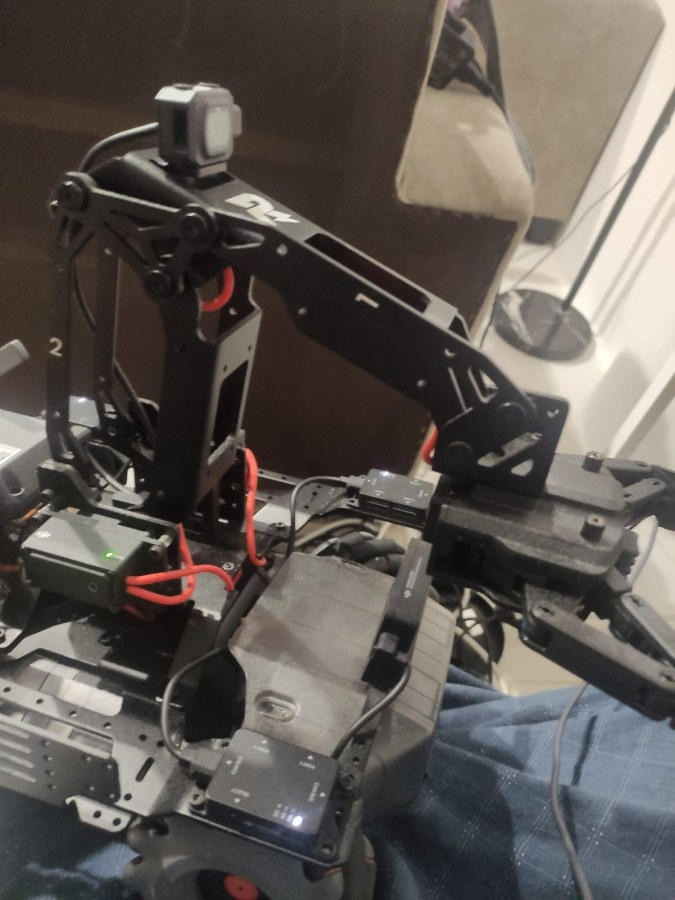
\includegraphics[height=6.2cm]{figures/photo_arm_side.jpg}
\caption{Side view: camera on the arm link, gripper at the front.}\end{subfigure}\hfill
\begin{subfigure}{0.31\linewidth}\centering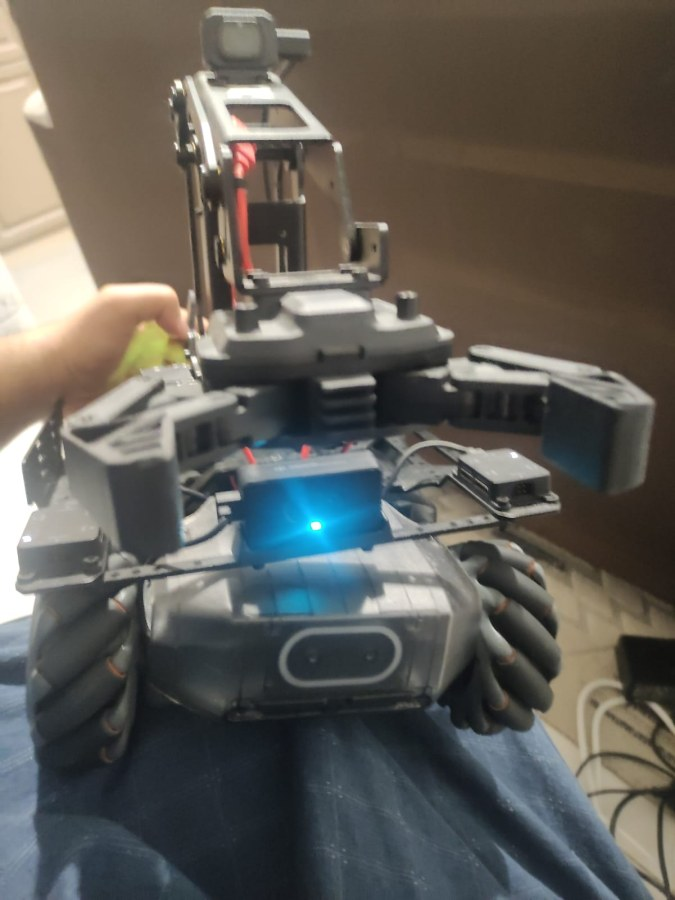
\includegraphics[height=6.2cm]{figures/photo_front_tof.jpg}
\caption{Front view: the ToF sensor (blue light) on the top front rail, under the gripper.}\end{subfigure}\hfill
\begin{subfigure}{0.31\linewidth}\centering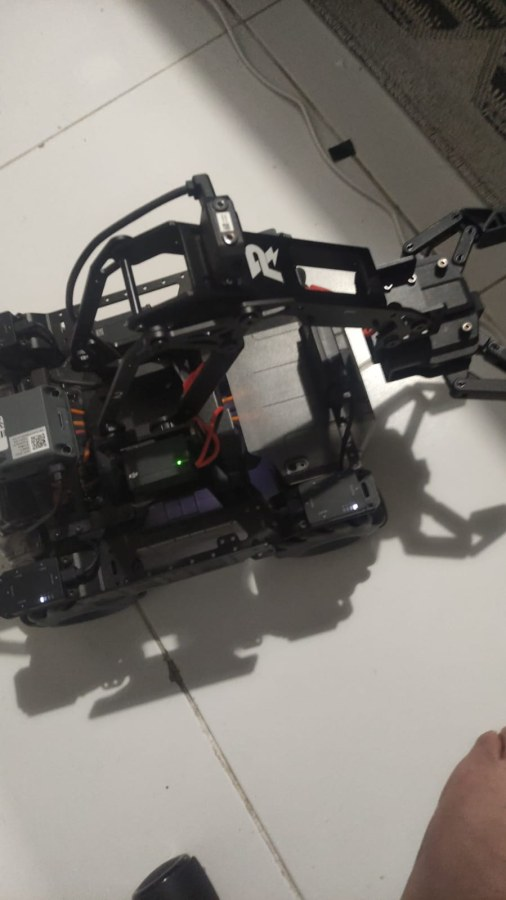
\includegraphics[height=6.2cm]{figures/photo_top_view.jpg}
\caption{Top view: arm and gripper over the front rail.}\end{subfigure}
\caption{Arm and ToF arrangement of the robot used (photos by the student). The low end effector pose of the
assignment would press the gripper onto the ToF sensor, so the arm was set by hand about 2\,cm above it.}
\label{fig:photos}
\end{figure}

\isub{\faRulerCombined}{Camera geometry: ground range, not slant range}
\label{sec:geom}
\label{sec:tf}

\begin{figure}[H]
\centering
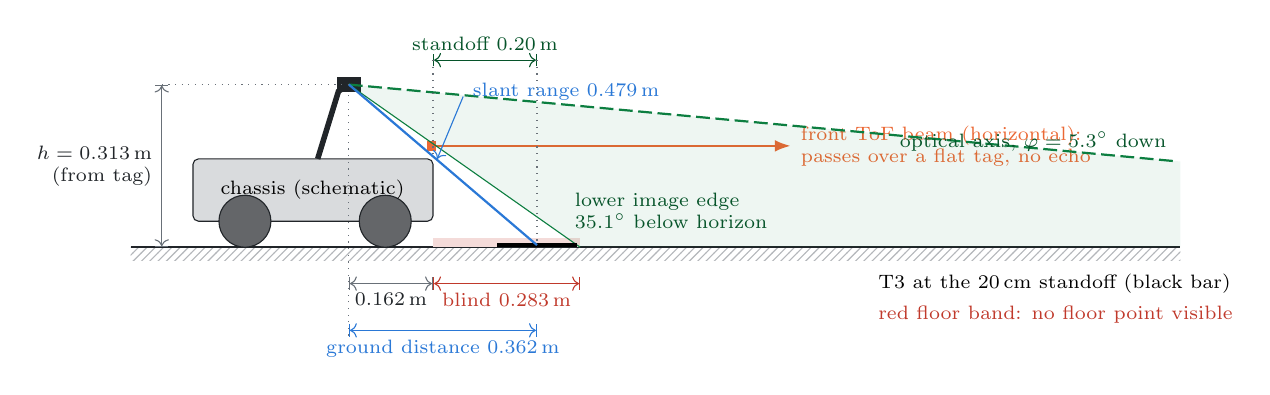
\begin{tikzpicture}[x=6.6cm,y=6.6cm,font=\small]
  % floor
  \fill[pattern=north east lines,pattern color=muted!50] (-0.42,-0.025) rectangle (1.6,0);
  \draw[ink,thick] (-0.42,0) -- (1.6,0);
  % blind zone on the floor
  \fill[accred!18] (0.162,0) rectangle (0.445,0.018);
  % chassis (schematic)
  \draw[ink,fill=muted!25,rounded corners=2pt] (-0.30,0.05) rectangle (0.162,0.17);
  \foreach \x in {-0.20,0.07} \draw[ink,fill=ink!70] (\x,0.05) circle (0.05);
  \node[font=\scriptsize] at (-0.07,0.11) {chassis (schematic)};
  % arm post and camera
  \draw[ink,line width=2pt] (-0.06,0.17) -- (-0.02,0.30) -- (0,0.313);
  \draw[ink,fill=ink] (-0.022,0.300) rectangle (0.022,0.326);
  % ToF beam
  \fill[accorange] (0.150,0.185) rectangle (0.168,0.205);
  \draw[accorange,thick,-{Latex[length=2mm]}] (0.168,0.195) -- (0.85,0.195)
     node[right,font=\scriptsize,align=left]{front ToF beam (horizontal):\\passes over a flat tag, no echo};
  % optical axis and lower FOV edge
  \draw[kfupm,thick,dash pattern=on 5pt off 2pt] (0,0.313) -- ($(0,0.313)+(-5.3:1.6)$) node[above left,font=\scriptsize,text=kfupmdark]{optical axis, $\varphi=5.3^\circ$ down};
  \draw[kfupm] (0,0.313) -- (0.445,0);
  \fill[kfupm,opacity=0.07] (0,0.313) -- (0.445,0) -- (1.6,0) -- (1.6,0.165) -- cycle;
  \node[font=\scriptsize,text=kfupmdark,align=left] at (0.62,0.07) {lower image edge\\$35.1^\circ$ below horizon};
  % tag at the standoff and slant vs ground range
  \fill[black] (0.362-0.0775,0) rectangle (0.362+0.0775,0.008);
  \draw[accblue,thick] (0,0.313) -- (0.362,0.004);
  \node[font=\scriptsize,text=accblue,align=left,anchor=west] at (0.22,0.30) {slant range 0.479\,m};
  \draw[accblue,->] (0.22,0.29) -- (0.17,0.17);
  % dimensions
  \draw[|<->|,muted] (-0.36,0) -- node[left,font=\scriptsize,text=ink,align=right]{$h=0.313$\,m\\(from tag)} (-0.36,0.313);
  \draw[dotted,muted] (-0.36,0.313) -- (0,0.313);
  \draw[|<->|,muted] (0,-0.07) -- node[below,font=\scriptsize,text=ink]{0.162\,m} (0.162,-0.07);
  \draw[|<->|,accblue] (0,-0.16) -- node[below,font=\scriptsize,text=accblue]{ground distance 0.362\,m} (0.362,-0.16);
  \draw[|<->|,accred] (0.162,-0.07) -- node[below,font=\scriptsize,text=accred]{blind 0.283\,m} (0.445,-0.07);
  \draw[|<->|,kfupmdark] (0.162,0.36) -- node[above,font=\scriptsize,text=kfupmdark]{standoff 0.20\,m} (0.362,0.36);
  \draw[dotted,muted] (0.162,0.36) -- (0.162,0.17); \draw[dotted,muted] (0.362,0.36) -- (0.362,0.01);
  \draw[dotted,muted] (0,-0.17) -- (0,0.30);
  \node[font=\scriptsize,anchor=west] at (1.0,-0.07) {T3 at the 20\,cm standoff (black bar)};
  \node[font=\scriptsize,anchor=west,text=accred] at (1.0,-0.13) {red floor band: no floor point visible};
\end{tikzpicture}
\caption{Side view of the camera geometry at the arm pose used (to scale, chassis schematic). Distances are
measured from the chassis front. At the standoff the tag is already below the image, and its slant range from the
camera is 0.479\,m.}
\label{fig:geom}
\end{figure}

\lead{The driver's arm TF is wrong for this arm.} The TF chain \code{base_link} $\rightarrow$
\code{camera_optical_link} published by the driver put the optical axis $18^\circ$ \emph{up} after the A2 arm move and
$22^\circ$ up with the arm resting on the ToF sensor, while the floor tag showed the same camera $15.9^\circ$
\emph{down}; with the $18^\circ$ TF the floor tag even came out 0.378\,m above the camera (\code{notes/lab_log.md}). The detector therefore does not use TF
(\code{extrinsics: tag}); it measures the camera pose from the floor tag itself.

\lead{Camera height and pitch from one floor tag} (\code{camera_from_floor_tag} in \code{geometry.py}).
pupil-apriltags returns the tag pose $(\mathbf R,\mathbf t)$ in the optical frame ($x$ right, $y$ down, $z$ forward).
A tag lying flat has its normal along the floor normal, so with $\mathbf n=\pm\mathbf R_{:,3}$ oriented toward the camera:
\begin{equation}
h=-\mathbf n^{T}\mathbf t,\qquad \varphi=\arcsin(-n_z),\qquad \text{roll}=\operatorname{atan2}(n_x,\,-n_y).
\end{equation}
No arm model or TF is needed. At the final arm pose this gave $h\approx0.313$\,m and $\varphi=5.3^\circ$ (roll within
$\pm0.4^\circ$), now fixed parameters of the detector.

\lead{Ground range and bearing} (\code{camera_to_level}). The tag center $\mathbf p=(x,y,z)$ is rotated into a level
frame at the camera, and the calibrated offset to the chassis front is applied:
\begin{equation}
\begin{aligned}
p_{fwd}&=z\cos\varphi-y\sin\varphi, \qquad p_{left}=-x,\\
d&=s\,p_{fwd}+o,\quad s=1.0,\ o=-0.162\text{\,m},\qquad \theta=\operatorname{atan2}(p_{left},\,p_{fwd}).
\end{aligned}
\end{equation}

\begin{bluebox}{\faRulerHorizontal\ \ Why the slant range must not be used for the brake}
\small
\begin{itemize}
  \item The straight-line range $\|\mathbf p\|$ contains the camera height. At the 20\,cm standoff the ground distance
        from the camera is $0.20+0.162=0.362$\,m but the slant range is $\sqrt{0.362^2+0.313^2}=0.479$\,m.
  \item Using the slant range with the same front offset would read $d=0.317$\,m at the standoff: the robot would
        brake about 11.7\,cm late, at roughly 8\,cm from the tag. The offline test
        \code{test_slant_range_overshoots_standoff} checks the same effect for the note example (0.32\,m read at 0.20\,m).
  \item The bearing error of the tilted camera is small; the range error is not.
\end{itemize}
\end{bluebox}

\isub{\faEye}{Range calibration and detection range}
\begin{itemize}
  \item \textbf{Tag:} printed T3 measured with a ruler: 155\,mm black edge (printer scale about 98\,\%), so
        \code{tag_size} $=0.155$\,m. Camera at 720p ($f_x=628.6$, $f_y=625.8$\,px).
  \item \textbf{Calibration:} T3 at tape distances from the chassis front; \code{tools/tag_range_probe.py} averaged 5\,s of
        detections. Rows 3 to 6 of \code{data/calibration/tag_range.csv} (1.20, 1.50, 0.60, 1.00\,m, 01:00:44 to
        01:07:34) were taken at the final arm pose, after the router-mode restart and before the pose was saved at 01:10;
        rows 1 and 2 belong to an earlier pose and are not used.
  \item \textbf{Model:} with the horizontal camera distance re-derived from the logged slant range and a camera height of
        0.310\,m, the offsets (tape minus camera) are $-0.0991$, $-0.1621$, $-0.1675$ and $-0.1619$\,m. Their median,
        $-0.1620$\,m, is the configured $o$ with scale $1.0$. A least-squares line gives scale 1.0176 and offset
        $-0.1692$\,m, pulled by the 1.20\,m point. With $o=-0.162$\,m the estimate minus tape is $+0.1$, $+5.5$ and
        $-0.1$\,mm at 1.50, 0.60 and 1.00\,m; the 1.20\,m point is an outlier at $-63$\,mm, most likely a misplaced
        tag, and the median is insensitive to it.
  \item \textbf{Real range limit:} at the final pose T3 was detected at 1.50\,m at 3.8 detections/s and at 0.6 to
        1.0\,m at 13.6 to 14.8 detections/s; at 1.80\,m the probe printed ``NOT DETECTED in 8\,s'' while the detector
        processed about 14 frames/s (\code{notes/lab_log.md}, 01:03; the probe writes no CSV row on a miss).
        The range limit of this 155\,mm tag lies between 1.5 and 1.8\,m, so all floor runs start at 1.50\,m
        (Figure~\ref{fig:range}).
\end{itemize}

\begin{figure}[H]
\centering
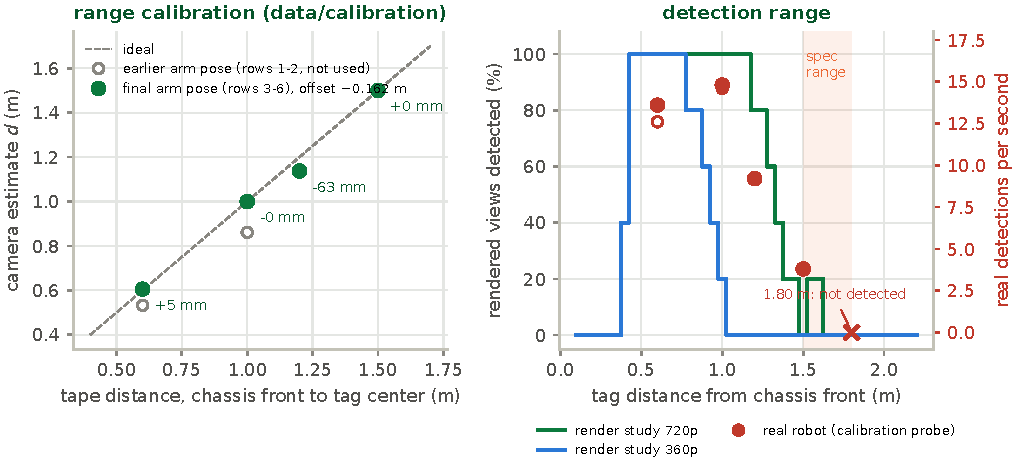
\includegraphics[width=\linewidth]{figures/p1_range.pdf}
\caption{Left: camera range estimate against the tape distance. Right: offline render study (real T3 bitmap on the
floor, calibrated 720p and 360p cameras at $h=0.313$\,m, $\varphi=5.3^\circ$, five in-plane tag rotations per
distance) and real detection rates. The render study is an ideal-image upper bound: at 720p every rotation is
detected from 0.45 to 1.15\,m and some up to 1.60\,m; 360p would stop near 1.0\,m.}
\label{fig:range}
\end{figure}

\isub{\faSyncAlt}{(ii) Search and centering finite state machine}
\label{sec:fsm}
The planner runs the state machine of Figure~\ref{fig:fsm} with the parameters of Table~\ref{tab:fsm}; the brake
conditions are detailed in Section~\ref{sec:brake}.

\begin{figure}[H]
\centering
\begin{tikzpicture}[font=\small]
  \node[stnode=SEARCHING] (S) at (0,0) {\textbf{\textcolor{cSEARCHING}{SEARCHING}}\\[1pt]\footnotesize
     $v=0$\\$\omega=\pm0.30$\,rad/s toward the\\side where T3 was last seen};
  \node[stnode=ALIGNING] (A) at (8.4,0) {\textbf{\textcolor{cALIGNING}{ALIGNING}}\\[1pt]\footnotesize
     $v=0$\\$\omega=1.0\,\theta$, $0.10\le|\omega|\le0.30$\,rad/s};
  \node[stnode=CHASING] (C) at (8.4,-4.0) {\textbf{\textcolor{cCHASING}{CHASING}}\\[1pt]\footnotesize
     $v=\dot x_{ref}(t)$ (cubic plan)\\$\omega=\omega_{ref}+0.8\,\theta$, $|\omega|\le0.30$};
  \node[stnode=ARRIVED] (R) at (0,-4.0) {\textbf{\textcolor{cARRIVED}{ARRIVED}}\\[1pt]\footnotesize
     active brake\\$v=0$, $\omega=0$ held};
  \draw[tr] ([yshift=4mm]S.east) -- node[trl,above=1pt]{T3 detected (age $\le0.45$\,s)} ([yshift=4mm]A.west);
  \draw[tr] ([yshift=-4mm]A.west) -- node[trl,below=1pt]{T3 hidden $>0.45$\,s} ([yshift=-4mm]S.east);
  \draw[tr] (A) -- node[trl,right=2pt,align=left]{$|\theta|\le0.18$\,rad on 3 consecutive\\detections: fix $d_0$, solve\\
     the cubic, start the clock} (C);
  \draw[tr] (C.north west) -- node[trl,sloped,above=1pt]{hidden $>2.0$\,s and $>0.25$\,m to go} (S.south east);
  \draw[tr,color=cARRIVED] (C) -- node[trl,above=2pt,align=center,text=ink,font=\scriptsize]{camera $d\le0.20$ \textbf{or} ToF $\le0.20$\\
     \textbf{or} odom.\ $\ge d_0-0.20$ \textbf{or} $t\ge T$} (R);
  \draw[tr,color=cARRIVED] (R.south west) .. controls +(-1.0,-0.9) and +(1.0,-0.9) .. (R.south east)
     node[pos=0.5,below,font=\scriptsize,text=ink]{every tick};
  \draw[tr,color=muted] (-2.3,1.35) node[above,font=\scriptsize,text=ink,align=center]{start: arm within\\6\,mm of saved pose} -- (S.north west);
  \node[draw=alert,dashed,rounded corners=3pt,font=\scriptsize,align=left,text width=4.1cm,fill=alert!4] at (4.2,-5.7)
     {\faShieldAlt\ any state: arm moved $>6$\,mm $\rightarrow$ ARRIVED. Every exit path (end, Ctrl+C, exception)
      sends zero velocity.};
\end{tikzpicture}
\caption{Supervisory state machine of \code{mission.py}, run by \code{flatness_planner} at 20\,Hz.
$\theta$ is the tag bearing ($+$ left), $d$ the ground range from the chassis front.}
\label{fig:fsm}
\end{figure}

\begin{table}[H]
\centering\small
\rowcolors{2}{kfupmlight}{white}
\begin{tabularx}{\linewidth}{@{}l c >{\raggedright\arraybackslash}X@{}}
\rowcolor{kfupm}\hd{Parameter} & \hd{Value} & \hd{Role}\\
\code{lost_timeout} & 0.45\,s & tag counts as hidden after this age (assignment value) in SEARCHING and ALIGNING\\
\code{search_rate} & 0.30\,rad/s & in-place sweep, sign from the last seen bearing (default CCW)\\
\code{align_tol}, \code{align_settle} & 0.18\,rad, 3 & centered when $|\theta|\le0.18$ on 3 consecutive detections\\
\code{align_gain}, min, max & 1.0, 0.10, 0.30\,rad/s & proportional turn; the minimum overcomes the chassis dead band\\
\code{chase_gain} & 0.8\,rad/s per rad & bearing correction added to the plan's $\omega_{ref}=0$ while T3 is visible\\
\code{chase_lost_timeout} & 2.0\,s & dropouts tolerated while chasing (about 4 detections/s at 1.5\,m)\\
\code{blind_zone} & 0.25\,m & remaining planned distance below which losing T3 is expected and ignored\\
\code{standoff}, \code{tof_brake} & 0.20\,m, 0.20\,m & brake thresholds; ToF readings below 0.02\,m are ignored\\
\end{tabularx}
\caption{State machine parameters (\code{MissionParams} in \code{mission.py}).}
\label{tab:fsm}
\end{table}

\begin{keybox}{\faCompass\ \ Why the robot aligns in place before translating}
\small
\begin{itemize}
  \item \textbf{The plan is only valid for a tag straight ahead.} The flat output is built in the robot frame at the
        chase start with $y(t)\equiv0$, a straight line along body $+X$. If the tag sits at bearing $\theta_0$, the
        plan ends $d_0\sin\theta_0$ to the side of it: 0.23\,m for $\theta_0=0.18$\,rad at $d_0=1.27$\,m, and
        0.95\,m for the $43.7^\circ$ (at $d=1.37$\,m) at which T3 first appeared in the final run. Centering first makes the straight
        flat output (zero curvature, $\omega_{ref}=0$) the right path; the remaining small error is removed by the bearing
        feedback.
  \item \textbf{It keeps the tag in view.} The half field of view is about $45^\circ$ and T3 is detected only up to about
        1.5\,m, with 3.8 detections/s at 1.5\,m. A turn while translating moves the tag across the image by rotation
        and parallax at once, so a tag near the edge leaves the view; motion blur also lowers the detection rate at
        the range limit. In-place rotation keeps the distance constant, so the tag stays at a detectable range while
        it moves to the image center, where the pose estimate is best.
  \item \textbf{It prevents trajectory drift.} Pure rotation and pure translation are the two motions the chassis
        tracks best; combined turning and driving adds roller slip and heading error to the odometry. The odometry
        stop criterion (straight distance $\ge d_0-0.20$) and the plan time $T$ both assume a straight path.
  \item \textbf{$d_0$ is measured at its best.} $d_0$ fixes the goal and the horizon $T$. It is taken when the tag is
        centered and the robot is still, not from a moving, off-center view.
\end{itemize}
\end{keybox}

\isub{\faStopCircle}{(iii) Standoff braking}
\label{sec:brake}
CHASING switches to ARRIVED on the first of four conditions, checked every 50\,ms tick before a command is sent:
\begin{enumerate}
  \item \textbf{camera} $d\le0.20$\,m while the tag is visible (assignment requirement),
  \item \textbf{front ToF} range $\le0.20$\,m (assignment requirement; readings $\le0.02$\,m are treated as no echo),
  \item \textbf{odometry}: straight distance from the chase start $\ge d_0-0.20$,
  \item \textbf{plan time}: $t\ge T$; the plan itself ends at $\dot x(T)=0$, so this is a smooth stop.
\end{enumerate}
ARRIVED then sends $v=0$, $\omega=0$ on every tick, keeps logging (3\,s of zero rows), and the node sends zero velocity
again on shutdown, on Ctrl+C and on exceptions.

\begin{warnbox}
\small\textbf{\color{warn}\faEyeSlash\ The camera cannot see the tag at the standoff}
\begin{itemize}
  \item With $\varphi=5.3^\circ$ and a $29.8^\circ$ half field of view below the axis, the lowest image row meets the floor
        0.283\,m from the chassis front; the whole 155\,mm tag is in view only beyond about 0.36\,m
        (Figure~\ref{fig:geom}). The last detections of the three floor runs were at 0.391, 0.397 and 0.400\,m.
  \item Condition 1 is implemented as specified, but at this arm pose it cannot fire; it would with the steeper
        assignment pose. A flat floor tag gives no ToF echo (the ToF read 0.382 to 0.865\,m during the final run), so
        condition 2 is the obstacle guard.
  \item The final approach is therefore carried by the plan and the odometry (conditions 3 and 4). Losing the tag
        within the last \code{blind_zone} of the plan does not abort the chase. All three floor runs stopped on these
        conditions and measured 21, 20 and 20\,cm with the tape (Section~\ref{sec:results}).
\end{itemize}
\end{warnbox}

\isub{\faFilm}{Implementation hint: preventing video stalls}
The hint targets a script that pulls frames with \code{cap.grab()} from an FFmpeg decoder: if frames are grabbed
faster than the decoder recycles its buffers, \code{av_frame_get_buffer} runs out of memory and the stream stalls.
This package has no grab loop, and it handles the same problem as follows:
\begin{itemize}
  \item \textbf{The driver owns the decoder.} \code{robomaster_ros} decodes the H.264 stream and publishes raw
        \code{camera/image_color}. The detector never holds a decoder buffer, it only receives ROS messages.
        (PyAV is not installed, which the driver reports as ``FFmpeg not available''; raw images still publish.)
  \item \textbf{Newest frame only.} The image callback stores only the latest message; a 15\,Hz timer takes it and
        clears the slot. A slow detection drops frames instead of queuing them, which is what the sleep between
        \code{grab()} calls achieves in the hint. During the final run the detector processed 13.0 to 14.4 frames/s.
  \item \textbf{Watchdog.} If no image arrives for 2\,s, the detector re-creates its camera subscriptions, which recovers
        the stream after a driver reconnect (logged as ``No camera image for 2.4\,s: re-subscribing'').
\end{itemize}

%======================== 3. PROBLEM 2: FLATNESS ===============================
\isec{\faRoute}{Problem 2: Differential Flatness Trajectory Generation}

\isub{\faCalculator}{(i) Flat output and algebraic inversion}
The pursuit is planned for a unicycle model in the mission frame, which is how the chassis is commanded here
(forward speed $v$ and yaw rate $\omega$ only, eq.~(4)):
\begin{equation}
\dot x=v\cos\psi,\qquad \dot y=v\sin\psi,\qquad \dot\psi=\omega .
\end{equation}
The position $z(t)=[x(t),\,y(t)]^T$ is a flat output \cite{fliess,murray,lectures}: every state and input follows from $z$ and its derivatives
without integrating anything. The heading is the direction of the velocity, $\psi=\operatorname{atan2}(\dot y,\dot x)$,
and differentiating it gives the inputs:

\begin{keybox}{\faCalculator\ \ Flat inversion (eq.~1 of the assignment)}
\begin{equation}
v(t)=\sqrt{\dot x(t)^2+\dot y(t)^2},\qquad
\omega(t)=\dot\psi(t)=\frac{\dot x(t)\,\ddot y(t)-\dot y(t)\,\ddot x(t)}{\dot x(t)^2+\dot y(t)^2}.
\label{eq:flat}
\end{equation}
\end{keybox}
\begin{itemize}
  \item \textbf{Singularity:} at $v=0$ the heading is not defined by $z$, and $\omega$ is $0/0$. \code{flat_inversion}
        returns $\omega=0$ when $\dot x^2+\dot y^2\le10^{-6}$; the plan never stops before $t=T$, where the sample is
        held at $v=0$, $\omega=0$.
  \item \textbf{This mission:} the tag is centered before the chase, so $y(t)\equiv0$ and eq.~(\ref{eq:flat}) reduces to
        $v=\dot x$, $\omega=0$. A curved plan (for example $y(T)\neq0$) would need no code change; the offline test
        \code{test_inversion_on_circle} checks eq.~(\ref{eq:flat}) on a circle.
\end{itemize}

\isub{\faTable}{(ii) Cubic polynomial matrix solution}
Each flat component is a cubic over the horizon $T$, $z_j(t)=\alpha_0^{[j]}+\alpha_1^{[j]}t+\alpha_2^{[j]}t^2+\alpha_3^{[j]}t^3$,
$j\in\{x,y\}$. Position and velocity at both ends (Table~\ref{tab:bc}) give four linear equations:
\begin{equation}
\underbrace{\begin{bmatrix}1&0&0&0\\0&1&0&0\\1&T&T^2&T^3\\0&1&2T&3T^2\end{bmatrix}}_{\mathbf A(T)}
\begin{bmatrix}\alpha_0^{[j]}\\\alpha_1^{[j]}\\\alpha_2^{[j]}\\\alpha_3^{[j]}\end{bmatrix}
=\begin{bmatrix}z_j(0)\\\dot z_j(0)\\z_j(T)\\\dot z_j(T)\end{bmatrix},
\qquad \det\mathbf A(T)=T^4\neq0 .
\label{eq:matrix}
\end{equation}
The system has a unique solution for every $T>0$. Solving it symbolically, with $\Delta=z_j(T)-z_j(0)$:
\begin{equation}
\alpha_0=z_j(0),\quad \alpha_1=\dot z_j(0),\quad
\alpha_2=\frac{3\Delta-\big(2\dot z_j(0)+\dot z_j(T)\big)T}{T^2},\quad
\alpha_3=\frac{-2\Delta+\big(\dot z_j(0)+\dot z_j(T)\big)T}{T^3}.
\end{equation}

\begin{table}[H]
\centering\small
\rowcolors{2}{kfupmlight}{white}
\begin{tabular}{@{}lcccc@{}}
\rowcolor{kfupm}\hd{Component} & \hd{$z_j(0)$} & \hd{$\dot z_j(0)$} & \hd{$z_j(T)$} & \hd{$\dot z_j(T)$}\\
$x$ (toward the tag) & 0 & 0.06\,m/s & $d_0-0.20$ & 0\\
$y$ (left) & 0 & 0 & 0 & 0\\
\end{tabular}
\caption{Boundary conditions of the assignment, in the robot frame fixed at the start of CHASING. With all $y$ values
zero, $\bm\alpha_y=\mathbf 0$.}
\label{tab:bc}
\end{table}

The implementation solves eq.~(\ref{eq:matrix}) numerically with \code{numpy.linalg.solve}, exactly as required
(\code{rm_flatness_nav/flatness.py}, verbatim):
\begin{lstlisting}[style=py]
def solve_flat_polynomial(z0, zdot0, zf, zdotf, T):
    """Cubic coefficients [a0, a1, a2, a3] that meet position and velocity at t = 0 and t = T (eq. 2)."""
    A = np.array([
        [1.0, 0.0, 0.0, 0.0],
        [0.0, 1.0, 0.0, 0.0],
        [1.0, T, T**2, T**3],
        [0.0, 1.0, 2.0 * T, 3.0 * T**2],
    ])
    b = np.array([z0, zdot0, zf, zdotf], dtype=float)
    return np.linalg.solve(A, b)


def time_horizon(d0, v_max=V_MAX, standoff=STANDOFF, t_min=T_MIN):
    """T = max(4, 1.6 (d0 - 0.20) / v_max) (eq. 3). The 1.6 factor keeps the cubic's peak speed below v_max."""
    return max(t_min, 1.6 * (d0 - standoff) / v_max)
\end{lstlisting}
\begin{itemize}
  \item \code{FlatTrajectory(d0)} calls it once per component when CHASING starts:
        \code{alpha_x = solve_flat_polynomial(0, 0.06, d0 - 0.20, 0, T)} and
        \code{alpha_y = solve_flat_polynomial(0, 0, 0, 0, T)}.
  \item Every 50\,ms tick, \code{sample(t)} evaluates $x,\dot x,\ddot x$ (and the same for $y$) and applies
        eq.~(\ref{eq:flat}); the result is the reference $(v,\omega)$ sent to the state machine.
\end{itemize}

\begin{table}[H]
\centering\small
\rowcolors{2}{kfupmlight}{white}
\begin{tabularx}{\linewidth}{@{}>{\raggedright\arraybackslash}Xccccccc@{}}
\rowcolor{kfupm}\hd{Case} & \hd{$d_0$ (m)} & \hd{$T$ (s)} & \hd{$\alpha_0^{[x]}$} & \hd{$\alpha_1^{[x]}$} & \hd{$\alpha_2^{[x]}$} & \hd{$\alpha_3^{[x]}$} & \hd{peak $\dot x$ (m/s)}\\
% Generated by analysis/plot_flatness.py (solve_flat_polynomial).
final run, 1st chase (cut at 10.45 s) & 1.440 & 12.40 & $0$ & $0.06$ & $1.452\times10^{-2}$ & $-9.105\times10^{-4}$ & 0.1371\\
final run, chase to the stop & 1.269 & 10.69 & $0$ & $0.06$ & $1.684\times10^{-2}$ & $-1.225\times10^{-3}$ & 0.1371\\
run 011925, last chase & 1.365 & 11.65 & $0$ & $0.06$ & $1.545\times10^{-2}$ & $-1.032\times10^{-3}$ & 0.1371\\
run 012232, last chase & 1.375 & 11.75 & $0$ & $0.06$ & $1.532\times10^{-2}$ & $-1.014\times10^{-3}$ & 0.1371\\
spec lower bound & 1.500 & 13.00 & $0$ & $0.06$ & $1.385\times10^{-2}$ & $-8.284\times10^{-4}$ & 0.1371\\
spec upper bound & 1.800 & 16.00 & $0$ & $0.06$ & $1.125\times10^{-2}$ & $-5.469\times10^{-4}$ & 0.1371\\

\end{tabularx}
\caption{Coefficients $\bm\alpha_x$ from \code{solve_flat_polynomial} (units m, m/s, m/s$^2$, m/s$^3$) for the measured
$d_0$ of the floor runs and for the two ends of the assignment range. $\bm\alpha_y=\mathbf 0$ in every case. Each plan
meets $x(T)=d_0-0.20$ and $\dot x(T)=0$ to machine precision.}
\label{tab:coeff}
\end{table}

For the chase that ended the final run ($d_0=1.269$\,m, $T=10.69$\,s):
\begin{equation}
x(t)=0.06\,t+1.684\times10^{-2}\,t^2-1.225\times10^{-3}\,t^3\ \text{m},\qquad y(t)=0,
\end{equation}
with $\ddot x(0)=0.0337$\,m/s$^2$ and $\ddot x(T)=-0.0449$\,m/s$^2$: a gentle start and a gentle stop.

\isub{\faHourglassHalf}{(iii) Time horizon scaling}
\begin{equation}
T=\max\!\left(4.0,\ \frac{1.6\,(d_0-0.20)}{v_{max}}\right),\qquad v_{max}=0.16\text{\,m/s}.
\label{eq:horizon}
\end{equation}

\begin{bluebox}{\faTachometerAlt\ \ Why the factor 1.6 keeps the cruise below $v_{max}$}
\small
\begin{itemize}
  \item Let $D=d_0-0.20$ and $c=D/T$ (the mean speed). With the coefficients above, $\dot x(t)$ is a downward parabola
        with its maximum at $t^*=-\alpha_2/(3\alpha_3)$ and
        \[ \dot x_{peak}=\dot x(0)+\frac{\big(3c-2\dot x(0)\big)^2}{3\big(2c-\dot x(0)\big)} . \]
  \item \textbf{Rest to rest} ($\dot x(0)=0$): $\dot x_{peak}=1.5\,c$. A cubic that starts and ends at rest needs a peak
        50\,\% above its mean speed, so $T=1.5\,D/v_{max}$ would just touch $v_{max}$; the factor 1.6 leaves a margin:
        $\dot x_{peak}=1.5/1.6\,v_{max}=0.150$\,m/s.
  \item \textbf{With the assignment start speed} $\dot x(0)=0.06$\,m/s and $c=v_{max}/1.6=0.1$\,m/s:
        $\dot x_{peak}=0.06+0.18^2/0.42=\mathbf{0.1371}$\,\textbf{m/s} $=0.857\,v_{max}$.
  \item The peak does not depend on $d_0$ as long as the second term of eq.~(\ref{eq:horizon}) is active, that is for
        $d_0>0.60$\,m, which covers the whole 1.5 to 1.8\,m range (Table~\ref{tab:coeff}, Figure~\ref{fig:profiles}).
        Longer distances get proportionally longer horizons, not higher speeds.
  \item The 4\,s floor applies only to short distances: it keeps the start and stop accelerations bounded when $D$ is
        small.
\end{itemize}
\end{bluebox}

\begin{figure}[H]
\centering
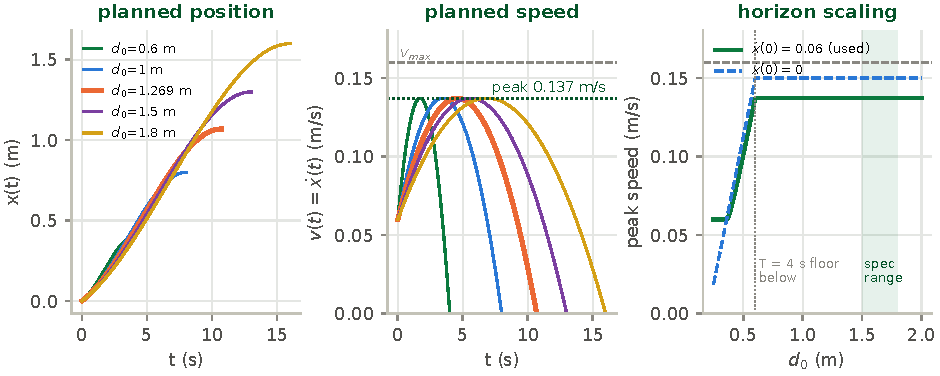
\includegraphics[width=\linewidth]{figures/p2_profiles.pdf}
\caption{Planned position and speed for several $d_0$ (bold: 1.269\,m, the final run) and the peak speed against $d_0$.
Every plan in the assignment range peaks at 0.137\,m/s, below $v_{max}$.}
\label{fig:profiles}
\end{figure}

\isub{\faChartLine}{Planned versus executed motion}
Figure~\ref{fig:planodom} compares the two plans of the final run with \code{/odom}, projected on the robot heading
at each chase start.
\begin{figure}[H]
\centering
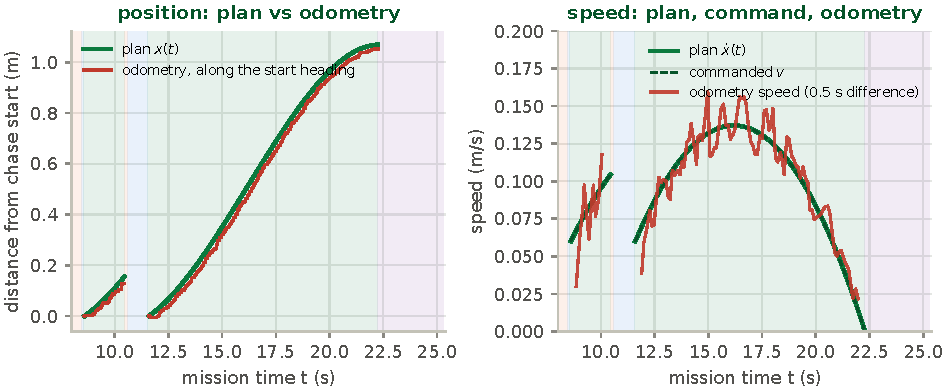
\includegraphics[width=\linewidth]{figures/p2_plan_vs_odom.pdf}
\caption{Final run: plan $x(t)$ and $\dot x(t)$ against the commanded speed and wheel odometry. The first chase
($d_0=1.440$\,m) was cut at 10.45\,s by a 2\,s detection gap; the second chase ($d_0=1.269$\,m) ran to the end of
its plan. Odometry speed is differenced over 5 \code{/odom} updates because single updates jitter over Wi-Fi.}
\label{fig:planodom}
\end{figure}
\begin{itemize}
  \item \textbf{Command = plan.} The commanded $v$ follows $\dot x_{ref}$ exactly; its maximum in the log is
        0.1371\,m/s at $t=16.05$\,s, the analytic peak.
  \item \textbf{Distance.} At the end of the plan the odometry shows 1.052\,m along the start heading and 1.060\,m in a
        straight line, against the planned 1.069\,m. Along the path, odometry trails the plan by 3.0\,cm on average
        (at most 4.8\,cm), the expected lag of a velocity-controlled chassis.
  \item \textbf{Lateral motion.} The chase began with T3 at $-9.1^\circ$ (inside the $\pm10^\circ$ tolerance). The
        bearing feedback turned the robot by $-6.7^\circ$ while driving, so it ended 13.2\,cm to the right of the
        start heading, toward the tag; the bearing at the last detection was $+0.012$\,rad.
  \item \textbf{Result.} The tape measured 20\,cm from the chassis front to the tag center after the stop.
\end{itemize}

%======================== 4. PROBLEM 3: VOLTAGES ===============================
\isec{\faBolt}{Problem 3: Motor Voltage Telemetry and Dynamics Logging}

\isub{\faCogs}{(i) Kinematics to wheel rates}
\begin{minipage}[c]{0.43\linewidth}
\centering
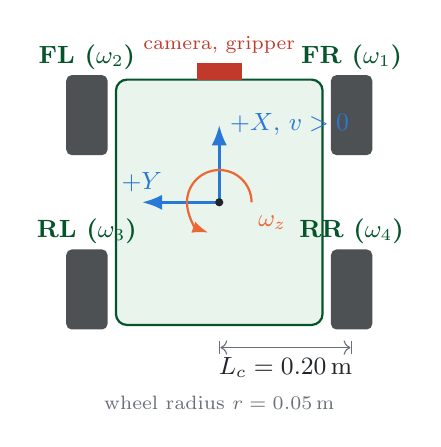
\begin{tikzpicture}[scale=0.82]
  \draw[kfupmdark,thick,fill=kfupmlight,rounded corners=4pt] (-1.6,-1.9) rectangle (1.6,1.9);
  \foreach \cx/\cy/\nm/\num in {-2.05/1.35/FL/2, 2.05/1.35/FR/1, -2.05/-1.35/RL/3, 2.05/-1.35/RR/4}{
    \fill[ink!80,rounded corners=2pt] (\cx-0.32,\cy-0.62) rectangle (\cx+0.32,\cy+0.62);
    \node[font=\small\bfseries,text=kfupmdark] at (\cx,\cy+0.9) {\nm\ ($\omega_{\num}$)};}
  % camera side at the top (+X)
  \fill[accred] (-0.35,1.9) rectangle (0.35,2.15);
  \node[font=\scriptsize,text=accred,above] at (0,2.15) {camera, gripper};
  \draw[-{Latex[length=2.6mm]},very thick,accblue] (0,0) -- (0,1.2) node[right,font=\small]{$+X$, $v>0$};
  \draw[-{Latex[length=2.6mm]},very thick,accblue] (0,0) -- (-1.2,0) node[above,font=\small]{$+Y$};
  \draw[-{Latex[length=2mm]},thick,accorange] (0.5,0) arc (0:250:0.5);
  \node[font=\small,text=accorange] at (0.82,-0.32) {$\omega_z$};
  \fill[ink] (0,0) circle (1.8pt);
  \draw[|<->|,muted] (0,-2.25) -- node[below,font=\small,text=ink]{$L_c=0.20$\,m} (2.05,-2.25);
  \node[font=\scriptsize,text=muted,align=center] at (0,-3.1) {wheel radius $r=0.05$\,m};
\end{tikzpicture}
\end{minipage}\hfill
\begin{minipage}[c]{0.55\linewidth}
\begin{keybox}{\faCogs\ \ Wheel rates (eq.~4)}
\vspace{-6pt}
\begin{equation}
\omega_1=\omega_4=\frac{v_x+L_c\,\omega_z}{r},\qquad
\omega_2=\omega_3=\frac{v_x-L_c\,\omega_z}{r}
\label{eq:wheels}
\end{equation}
\end{keybox}
\small
\begin{itemize}
  \item $1=$ FR, $2=$ FL, $3=$ RL, $4=$ RR. A counter-clockwise turn ($\omega_z>0$) speeds up the right side.
  \item It is the Mecanum inverse kinematics \cite{lynch} of Assessment~1 with $v_y=0$ and $l_x+l_y$ replaced by $L_c$. The
        A1 fit on logged data gave $R=51.0$\,mm and $l_x+l_y=204.7$\,mm, close to the $r$ and $L_c$ used here.
  \item Inputs are the \emph{commanded} $(v,\omega)$ in the mission frame, so $v>0$ (toward the tag) gives positive
        wheel rates.
\end{itemize}
\end{minipage}

\isub{\faBolt}{(ii) Motor armature voltage model}
\begin{keybox}{\faBolt\ \ Armature voltage (eq.~5), $K_v=0.38$\,V\,s/rad, $K_a=0.06$\,V\,s$^2$/rad}
\vspace{-6pt}
\begin{equation}
V_i(t)=\underbrace{K_v\,\omega_i(t)}_{\text{back-EMF}}+\underbrace{K_a\,\frac{\omega_i(t)-\omega_i(t-\Delta t)}{\Delta t}}_{\text{inertia}},
\qquad i\in\{1,2,3,4\},\qquad \Delta t=0.05\text{\,s}.
\label{eq:volt}
\end{equation}
\end{keybox}
\begin{itemize}
  \item \textbf{Where it runs:} inside the 20\,Hz control tick of \code{flatness_planner}, right after the command is
        published. $\Delta t$ is the control period; the logged tick interval was $50.0\pm0.3$\,ms (47 to 53\,ms) in
        the final run. The previous rates start at zero.
  \item \textbf{Which $\omega_i$:} the rates of eq.~(\ref{eq:wheels}) from the commanded $(v,\omega)$. The model gives
        the voltage the motors need to realize the command; it is not a measurement of the ESC terminals.
  \item \textbf{Steady values:} in a pure search turn ($\omega=0.30$\,rad/s) $|\omega_i|=1.2$\,rad/s and
        $|V_i|=0.38\times1.2=0.456$\,V. At the peak cruise speed (0.137\,m/s, $\omega_i=2.74$\,rad/s) the back-EMF term
        is about 1.04\,V.
  \item \textbf{Logging:} every tick goes to \code{motor_voltage_full.csv}; every 1\,s one row is printed to the
        terminal and written to \code{motor_voltage_log.csv} (the deliverable).
\end{itemize}

\begin{lstlisting}[style=py]
def wheel_rates(vx, wz, r=R_WHEEL, lc=L_C):
    """[w1, w2, w3, w4] in rad/s from forward speed vx (m/s) and yaw rate wz (rad/s, CCW +) (eq. 4)."""
    w_fr = (vx + lc * wz) / r
    w_fl = (vx - lc * wz) / r
    return np.array([w_fr, w_fl, w_fl, w_fr])


def motor_voltages(w, w_prev, dt, kv=K_V, ka=K_A):
    """V_i = Kv w_i + Ka (w_i - w_i_prev) / dt (eq. 5)."""
    w = np.asarray(w, dtype=float)
    return kv * w + ka * (w - np.asarray(w_prev, dtype=float)) / dt
\end{lstlisting}

\isub{\faTable}{(iii) Live table and CSV logging: Table 1}
Table~\ref{tab:table1} lists every row of \code{motor_voltage_log.csv} of the final run, as written by the planner
(target T3, start 1.50\,m, robot turned away from the tag). The terminal printed the same five columns live.
Unlike the template of the assignment, the log starts in SEARCHING, because T3 was placed outside the initial view
to demonstrate the sweep.

\begin{table}[H]
\centering\small
\setlength{\tabcolsep}{5.5pt}
\renewcommand{\arraystretch}{1.08}
\rowcolors{2}{kfupmlight}{white}
\begin{tabular}{@{}r rrrr rr r l@{}}
\rowcolor{kfupm}\hd{$t$ (s)} & \hd{$V_1$ (V)} & \hd{$V_2$ (V)} & \hd{$V_3$ (V)} & \hd{$V_4$ (V)} & \hd{$v$ (m/s)} & \hd{$\omega$ (rad/s)} & \hd{$d$ (m)} & \hd{State}\\
% Generated by analysis/plot_voltage.py from data/runs/20261026_015001/motor_voltage_log.csv.
% Values copied verbatim (strings), do not edit by hand.
0 & 1.896 & $-1.896$ & $-1.896$ & 1.896 & 0.0000 & 0.3000 & n/a & \stbadge{SEARCHING}\\
1 & 0.456 & $-0.456$ & $-0.456$ & 0.456 & 0.0000 & 0.3000 & n/a & \stbadge{SEARCHING}\\
2 & 0.456 & $-0.456$ & $-0.456$ & 0.456 & 0.0000 & 0.3000 & n/a & \stbadge{SEARCHING}\\
3 & 0.456 & $-0.456$ & $-0.456$ & 0.456 & 0.0000 & 0.3000 & n/a & \stbadge{SEARCHING}\\
4 & 0.456 & $-0.456$ & $-0.456$ & 0.456 & 0.0000 & 0.3000 & n/a & \stbadge{SEARCHING}\\
5 & 0.456 & $-0.456$ & $-0.456$ & 0.456 & 0.0000 & 0.3000 & n/a & \stbadge{SEARCHING}\\
6 & 0.456 & $-0.456$ & $-0.456$ & 0.456 & 0.0000 & 0.3000 & 1.273 & \stbadge{ALIGNING}\\
7 & 0.456 & $-0.456$ & $-0.456$ & 0.456 & 0.0000 & 0.3000 & 1.300 & \stbadge{SEARCHING}\\
8 & 0.456 & $-0.456$ & $-0.456$ & 0.456 & 0.0000 & 0.3000 & 1.300 & \stbadge{SEARCHING}\\
9 & 0.583 & 0.583 & 0.583 & 0.583 & 0.0725 & 0.0000 & 1.440 & \stbadge{CHASING}\\
10 & 0.750 & 0.750 & 0.750 & 0.750 & 0.0953 & 0.0000 & 1.440 & \stbadge{CHASING}\\
11 & $-0.437$ & 0.437 & 0.437 & $-0.437$ & 0.0000 & $-0.2878$ & 1.267 & \stbadge{ALIGNING}\\
12 & 0.552 & 0.652 & 0.652 & 0.552 & 0.0744 & $-0.0532$ & 1.288 & \stbadge{CHASING}\\
13 & 0.847 & 0.729 & 0.729 & 0.847 & 0.1000 & 0.0222 & 1.193 & \stbadge{CHASING}\\
14 & 0.952 & 0.916 & 0.916 & 0.952 & 0.1205 & 0.0118 & 1.101 & \stbadge{CHASING}\\
15 & 1.029 & 1.005 & 1.005 & 1.029 & 0.1324 & 0.0067 & 0.963 & \stbadge{CHASING}\\
16 & 1.063 & 1.024 & 1.024 & 1.063 & 0.1371 & 0.0062 & 0.836 & \stbadge{CHASING}\\
17 & 0.997 & 1.031 & 1.031 & 0.997 & 0.1344 & 0.0036 & 0.690 & \stbadge{CHASING}\\
18 & 0.931 & 0.926 & 0.926 & 0.931 & 0.1243 & 0.0043 & 0.572 & \stbadge{CHASING}\\
19 & 0.807 & 0.784 & 0.784 & 0.807 & 0.1079 & 0.0074 & 0.456 & \stbadge{CHASING}\\
20 & 0.544 & 0.636 & 0.636 & 0.544 & 0.0821 & 0.0000 & 0.391 & \stbadge{CHASING}\\
21 & 0.337 & 0.337 & 0.337 & 0.337 & 0.0500 & 0.0000 & 0.391 & \stbadge{CHASING}\\
22 & 0.028 & 0.028 & 0.028 & 0.028 & 0.0105 & 0.0000 & 0.391 & \stbadge{CHASING}\\
23 & 0.000 & 0.000 & 0.000 & 0.000 & 0.0000 & 0.0000 & 0.391 & \stbadge{ARRIVED}\\
24 & 0.000 & 0.000 & 0.000 & 0.000 & 0.0000 & 0.0000 & 0.391 & \stbadge{ARRIVED}\\
25 & 0.000 & 0.000 & 0.000 & 0.000 & 0.0000 & 0.0000 & 0.391 & \stbadge{ARRIVED}\\

\end{tabular}
\caption{Chassis motor armature voltage log, target Tag 3, final run \code{20261026_015001} (verbatim rows of
\code{motor_voltage_log.csv}). $v$, $\omega$ are the commanded values of that tick. $d$ is the last camera range
received (it holds its value while T3 is not seen, and n/a before the first detection). $T_{stop}=22.30$\,s; from
$t=23$\,s all four voltages are 0.000\,V.}
\label{tab:table1}
\end{table}

\begin{figure}[H]
\centering
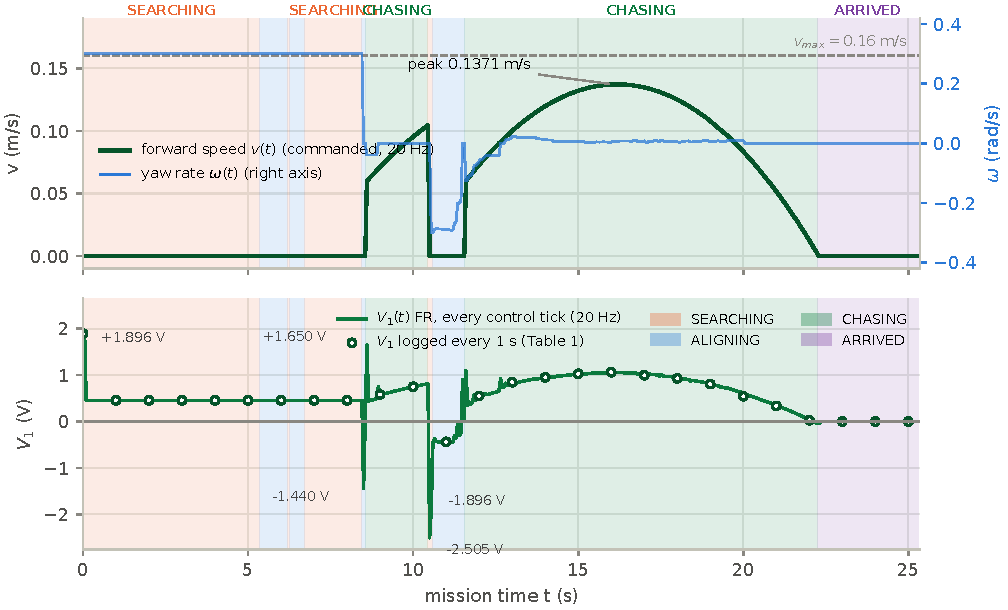
\includegraphics[width=\linewidth]{figures/p3_v_V1.pdf}
\caption{Forward speed $v(t)$ and motor voltage $V_1(t)$ (front right) over the final run, with the state machine
colored in the background. Top: commanded $v$ and $\omega$ at 20\,Hz. Bottom: $V_1$ at every control tick (line) and
the 1\,s rows of Table~\ref{tab:table1} (circles).}
\label{fig:vV1}
\end{figure}

\begin{figure}[H]
\centering
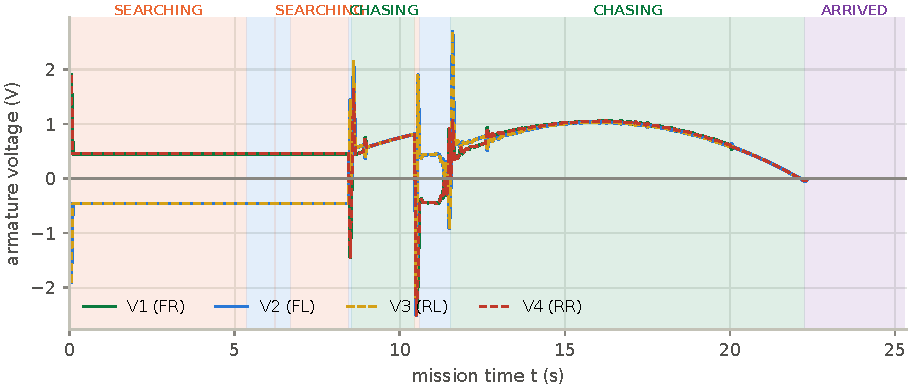
\includegraphics[width=\linewidth]{figures/p3_voltages_all.pdf}
\caption{All four armature voltages at 20\,Hz. Left and right pairs are equal ($V_1=V_4$, $V_2=V_3$) because eq.~(4)
has no lateral term; they differ only when $\omega\neq0$.}
\label{fig:vall}
\end{figure}

\begin{purplebox}{\faSearch\ \ Reading the voltage log}
\small
\begin{itemize}
  \item \textbf{Zero after the halt (confirmed).} The 1\,s rows at $t=23$, 24 and 25\,s are 0.000\,V on all motors. At
        20\,Hz the first ARRIVED tick (22.30\,s) carries $-0.041$\,V, the inertia term of the last speed decrement;
        the remaining 60 ticks are exactly 0.000\,V.
  \item \textbf{Search turn} (Figure~\ref{fig:vall}): $V_1=V_4=+0.456$\,V, $V_2=V_3=-0.456$\,V: the right side drives forward, the left side
        backward, the robot turns counter-clockwise.
  \item \textbf{Spikes are steps of the command.} Eq.~(\ref{eq:volt}) differentiates the command over one 50\,ms tick,
        so every step adds $K_a\Delta\omega_i/\Delta t$ for one tick:
        \begin{itemize}
          \item $t=0$: $0\rightarrow1.2$\,rad/s, $0.456+0.06\times1.2/0.05=\mathbf{1.896}$\,V (the first row of
                Table~\ref{tab:table1});
          \item 8.50\,s, centered: the turn stops, $-1.440$\,V on $V_1$;
          \item 8.60 and 11.60\,s, CHASING starts at $\dot x(0)=0.06$\,m/s (a step required by the boundary
                condition) plus the bearing correction: up to $+2.694$\,V on $V_2$;
          \item 10.50\,s, detection gap: the chase drops from 0.104\,m/s to rest, $-2.505$\,V on all motors.
        \end{itemize}
  \item \textbf{Smooth cruise.} Inside the plan the planned acceleration ($|\ddot x|\le0.045$\,m/s$^2$) adds at most $0.06\times0.0449/0.05=0.054$\,V; small
        changes of the bearing correction add up to 0.23\,V on single wheels. $V_1$ follows the speed profile and
        peaks at 1.063\,V in the $t=16$\,s row.
  \item \textbf{Negative voltage while braking.} In the last three CHASING ticks (22.15 to 22.25\,s) the deceleration
        term outweighs the back-EMF of the nearly stopped wheels: $-0.006$, $-0.023$, $-0.040$\,V. The motors oppose
        the motion: braking, which a real drive can do regeneratively.
  \item \textbf{Left and right voltages differ only while turning} or in the tick where a turn stops
        (rows 11 to 20: re-alignment and bearing correction, $|\omega|\le0.29$\,rad/s).
\end{itemize}
\end{purplebox}

%======================== 5. EXPERIMENTAL RESULTS ==============================
\isec{\faFlask}{Experimental Results}
\label{sec:results}

\isub{\faListOl}{Test progression}
New motion code reached the floor only after passing each stage of Figure~\ref{fig:ladder}; every stage is logged in
\code{data/}, and Table~\ref{tab:runs} lists all logged missions.

\begin{figure}[H]
\centering
\begin{tikzpicture}[node distance=3mm,
  stage/.style={draw=#1,fill=#1!8,line width=0.9pt,rounded corners=4pt,align=center,text width=2.6cm,
                minimum height=2.1cm,font=\footnotesize}]
  \node[stage=accblue] (s1) {\faVial\\[2pt]\textbf{Offline tests}\\36 pytest cases, closed-loop mission simulation};
  \node[stage=accgold,right=of s1] (s2) {\faEyeSlash\\[2pt]\textbf{Dry runs}\\\code{cmd_vel} remapped, robot never commanded};
  \node[stage=accorange,right=of s2] (s3) {\faCogs\\[2pt]\textbf{Wheels off}\\robot lifted, wheel directions and stop checked};
  \node[stage=kfupm,right=of s3] (s4) {\faRobot\\[2pt]\textbf{Floor runs}\\T3 at 1.50\,m, tape standoff after each stop};
  \node[stage=accpurple,right=of s4] (s5) {\faVideo\\[2pt]\textbf{Final run}\\filmed, Table~1, video};
  \foreach \pa/\pb in {s1/s2,s2/s3,s3/s4,s4/s5} \draw[arr] (\pa) -- (\pb);
\end{tikzpicture}
\caption{Validation ladder. The first test of each new motion behavior was done with the wheels off the ground.}
\label{fig:ladder}
\end{figure}

\begin{table}[H]
\centering\footnotesize
\setlength{\tabcolsep}{4pt}
\rowcolors{2}{kfupmlight}{white}
\begin{tabularx}{\linewidth}{@{}l>{\raggedright\arraybackslash}Xrcrrr>{\raggedright\arraybackslash}p{1.9cm}rr@{}}
\rowcolor{kfupm}\hd{Run} & \hd{Type} & \hd{Length (s)} & \hd{Chases} & \hd{$d_0$ (m)} & \hd{$T$ (s)} & \hd{Stop (s)} & \hd{Brake trigger} & \hd{Last $d$ (m)} & \hd{Tape}\\
% Generated by analysis/plot_run.py
\code{20261026_010948} & dry run, \code{cmd_vel} remapped & 11.2 & 1 & 0.999 & 7.99 & 8.15 & plan time $T$ & 1.000 & n/a\\
\code{20261026_011222} & wheels off the ground & 11.2 & 1 & 1.010 & 8.10 & 8.20 & plan time $T$ & 1.011 & n/a\\
\code{20261026_011631} & wheels off the ground & 10.4 & 1 & 0.924 & 7.24 & 7.40 & plan time $T$ & 0.405 & n/a\\
\code{20261026_011925} & floor run 1 & 20.1 & 5 & 1.365 & 11.65 & 17.10 & plan time $T$ & 0.397 & \textbf{21\,cm}\\
\code{20261026_012232} & floor run 2 & 16.4 & 2 & 1.375 & 11.75 & 13.35 & odometry & 0.400 & \textbf{20\,cm}\\
\code{20261026_013032} & dry run, \code{cmd_vel} remapped & 58.0 & 0 & n/a & n/a & n/a & no tag in view (search only) & n/a & n/a\\
\code{20261026_015001} & floor run 3 (final, filmed) & 25.3 & 2 & 1.269 & 10.69 & 22.30 & plan time $T$ & 0.391 & \textbf{20\,cm}\\

\end{tabularx}
\caption{Every logged mission. ``Chases'' counts the starts of CHASING ($d_0$ and $T$ are those of the last one).
``Last $d$'' is the last camera range received. The tape column is the standoff measured by the student after the
stop, chassis front to tag center (target 20\,cm).}
\label{tab:runs}
\end{table}

\begin{itemize}
  \item \textbf{Standoff accuracy:} 21, 20 and 20\,cm on the three floor runs, against a 20\,cm target.
  \item \textbf{Run 1 (\code{011925}):} the chase restarted four times in the first 5.4\,s. At 1.45\,m the tag gave about 4
        detections/s, so the 0.45\,s visibility rule kept declaring it lost. The chase dropout limit was raised (first
        to 1.5\,s) after this run.
  \item \textbf{Run 2 (\code{012232}):} one restart (SEARCHING at 2.0\,s, CHASING again at 2.2\,s) after a 1.6\,s detection gap caused by the start jolt; the
        brake came from odometry (1.177\,m covered for a 1.175\,m goal). The limit was then set to 2.0\,s.
  \item \textbf{Run 3 (\code{015001}, final):} one restart after a 2.0\,s gap at 10.45\,s, then a complete chase that
        ended on the plan time. Analysed in detail below.
  \item \textbf{Simulation:} the closed-loop test simulation stops 0.200\,m from the tag for straight, offset
        and hidden-tag starts, with a peak speed of 0.1371\,m/s.
\end{itemize}

\isub{\faStopwatch}{Final run timeline}
Figure~\ref{fig:tikztimeline} summarizes the final run; Figure~\ref{fig:timeline} shows the signals behind it and
Figure~\ref{fig:topview} the driven path.
\begin{figure}[H]
\centering
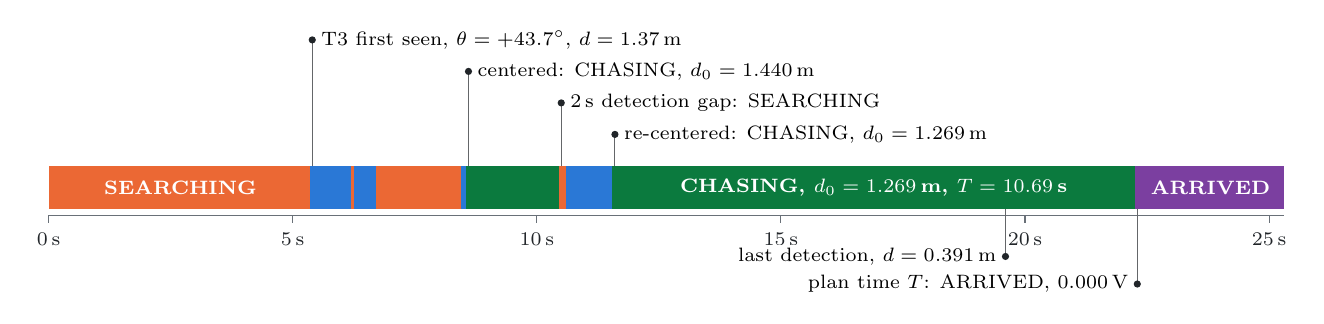
\begin{tikzpicture}[x=0.62cm,y=1cm]
  \foreach \ta/\tb/\st in {0/5.35/SEARCHING,5.35/6.20/ALIGNING,6.20/6.25/SEARCHING,6.25/6.70/ALIGNING,6.70/8.45/SEARCHING,
                        8.45/8.55/ALIGNING,8.55/10.45/CHASING,10.45/10.60/SEARCHING,10.60/11.55/ALIGNING,
                        11.55/22.25/CHASING,22.25/25.30/ARRIVED}
    \fill[fill=c\st] (\ta,0) rectangle (\tb,0.55);
  \node[white,font=\scriptsize\bfseries] at (2.7,0.275) {SEARCHING};
  \node[white,font=\scriptsize\bfseries] at (16.9,0.275) {CHASING, $d_0=1.269$\,m, $T=10.69$\,s};
  \node[white,font=\scriptsize\bfseries] at (23.8,0.275) {ARRIVED};
  \draw[muted] (0,-0.08) -- (25.3,-0.08);
  \foreach \tv in {0,5,10,15,20,25} {\draw[muted] (\tv,-0.08) -- (\tv,-0.18) node[below,font=\scriptsize,text=ink]{\tv\,s};}
  % events: early ones above the bar (earlier = higher), late ones below the axis
  \foreach \tv/\lvl/\txt in {5.40/4/{T3 first seen, $\theta=+43.7^\circ$, $d=1.37$\,m},
                           8.60/3/{centered: CHASING, $d_0=1.440$\,m},
                           10.50/2/{2\,s detection gap: SEARCHING},
                           11.60/1/{re-centered: CHASING, $d_0=1.269$\,m}}{
    \draw[ink!70] (\tv,0.55) -- (\tv,0.55+0.4*\lvl);
    \fill[ink] (\tv,0.55+0.4*\lvl) circle (1.3pt);
    \node[font=\scriptsize,anchor=west,fill=white,inner sep=1pt] at (\tv+0.12,0.55+0.4*\lvl) {\txt};}
  \foreach \tv/\lvl/\txt in {19.60/1/{last detection, $d=0.391$\,m},
                           22.30/2/{plan time $T$: ARRIVED, 0.000\,V}}{
    \draw[ink!70] (\tv,0) -- (\tv,-0.25-0.35*\lvl);
    \fill[ink] (\tv,-0.25-0.35*\lvl) circle (1.3pt);
    \node[font=\scriptsize,anchor=east,fill=white,inner sep=1pt] at (\tv-0.12,-0.25-0.35*\lvl) {\txt};}
\end{tikzpicture}
\caption{State timeline of run \code{20261026_015001} with the key events (times from the 20\,Hz log).}
\label{fig:tikztimeline}
\end{figure}

\begin{figure}[H]
\centering
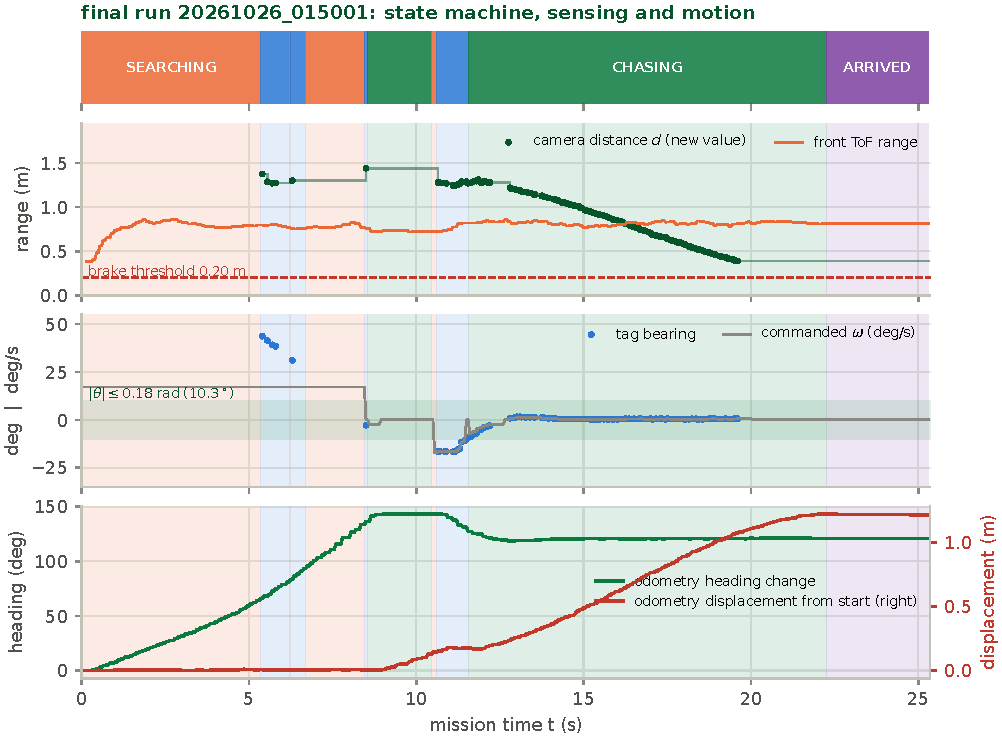
\includegraphics[width=\linewidth]{figures/p5_timeline.pdf}
\caption{Final run in detail. Camera range (new detections as dots) and ToF range; tag bearing with the
$\pm0.18$\,rad window and the commanded yaw rate; odometry heading change and displacement.}
\label{fig:timeline}
\end{figure}

\begin{itemize}
  \item \textbf{SEARCHING (0 to 5.35\,s):} counter-clockwise sweep at 0.30\,rad/s; odometry shows $65.8^\circ$ of
        rotation before T3 entered the image at its left edge ($+43.7^\circ$).
  \item \textbf{ALIGNING with flicker (5.35 to 8.55\,s):} at 1.3 to 1.4\,m the tag was at the edge of its range and of
        the image, so detections came and went and the state alternated with SEARCHING. Both states kept turning
        toward the tag (the search side follows the last bearing), so the sweep continued until T3 was centered
        ($\theta=-0.049$\,rad).
  \item \textbf{First chase (8.60 to 10.45\,s):} started from $d_0=1.440$\,m; a detection gap longer than 2.0\,s
        returned the robot to SEARCHING after 0.13\,m.
  \item \textbf{Re-alignment (10.50 to 11.55\,s):} the sweep went clockwise (last bearing negative), T3 reappeared
        at $-16.4^\circ$ ($-0.287$\,rad) and was centered in about 1\,s.
  \item \textbf{Final chase (11.60 to 22.25\,s):} $d_0=1.269$\,m, $T=10.69$\,s; from 12.8\,s about 13 new
        detections/s (gaps $\le0.2$\,s) until the tag left the image at 0.391\,m (19.60\,s); the plan carried the robot through the blind zone and
        ended at $t=T$. ARRIVED at 22.30\,s, tape standoff \textbf{20\,cm}.
\end{itemize}

\begin{figure}[H]
\centering
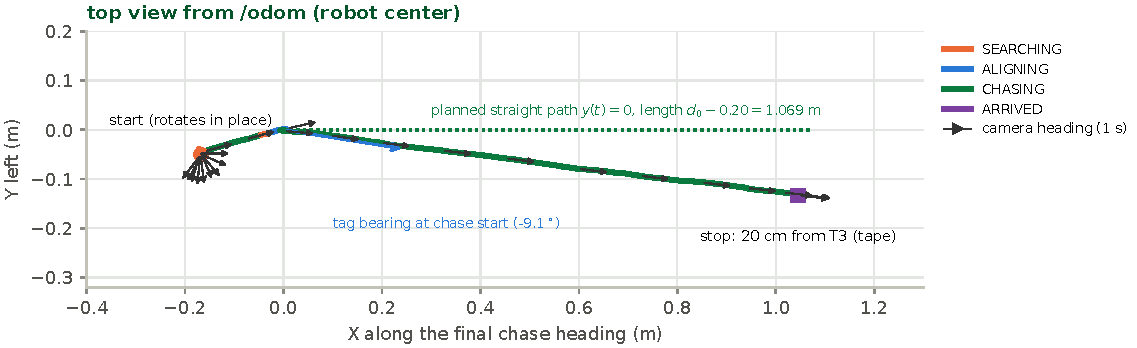
\includegraphics[width=\linewidth]{figures/p5_topview.pdf}
\caption{Path of the robot center from \code{/odom}, rotated so that the final chase starts at the origin along $+X$.
The in-place sweep appears as the cluster of heading arrows at the start; the final chase bends slightly right,
toward the tag that was at $-9.1^\circ$ when it started.}
\label{fig:topview}
\end{figure}

\isub{\faFilm}{Demonstration video}
\begin{itemize}
  \item \textbf{File:} \code{video/A2_demo_side_by_side.mp4}, 23.8\,s ($\le45$\,s), 1920$\times$480 at 30\,fps:
        \link{\videolink}{\faVideo\ demo video}.
  \item \textbf{Layout:} phone recording of the robot (left), robot camera with the T3 detection box (middle) and a top
        view of the driven path against the planned cubic $z(t)$ (right). The overlay shows mission time, state,
        $d$, $\theta$ and the command.
  \item \textbf{Content:} (a) sweep in place while T3 is hidden, (b) centering when T3 is spotted, (c) cruise and stop at
        20\,cm. Figure~\ref{fig:stills} shows one frame of each phase.
\end{itemize}

\begin{figure}[p]
\centering
\begin{subfigure}{\linewidth}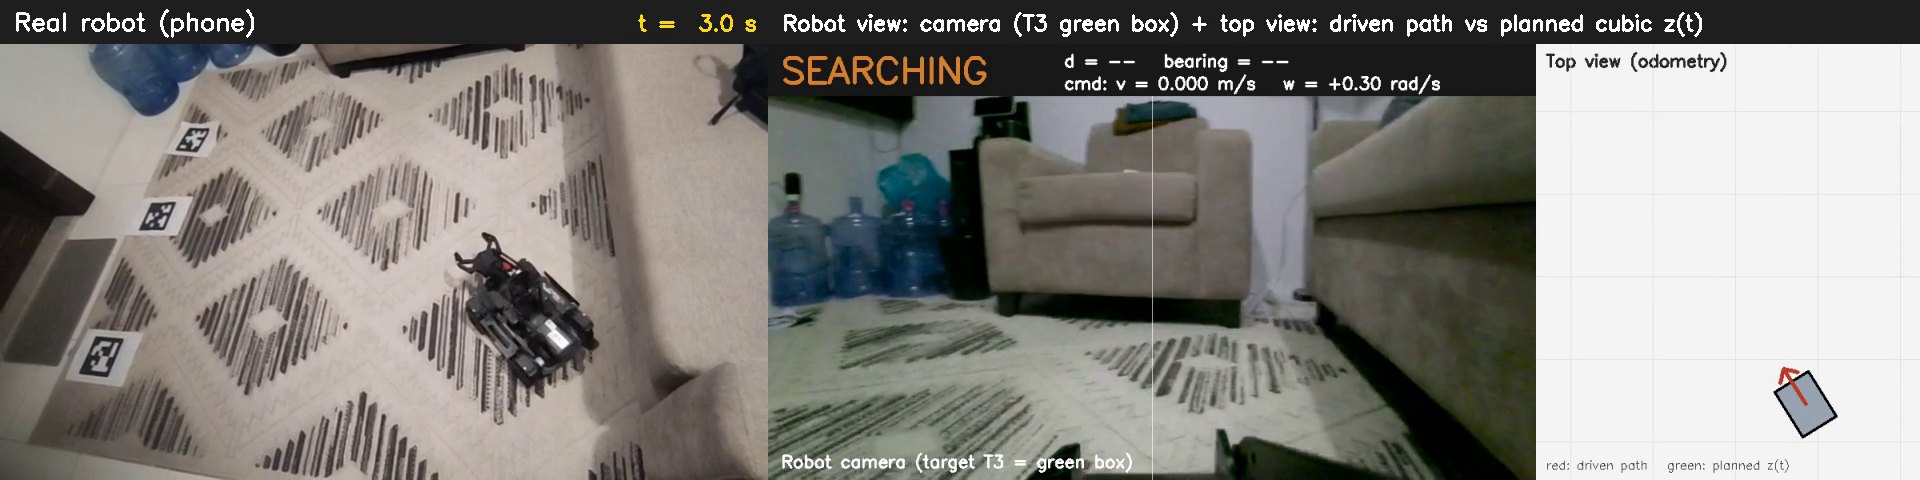
\includegraphics[width=\linewidth]{figures/still_searching.jpg}
\caption{SEARCHING, $t=3.0$\,s: sweeping counter-clockwise, T3 (left in the phone view) is outside the camera view.}\end{subfigure}\\[3pt]
\begin{subfigure}{\linewidth}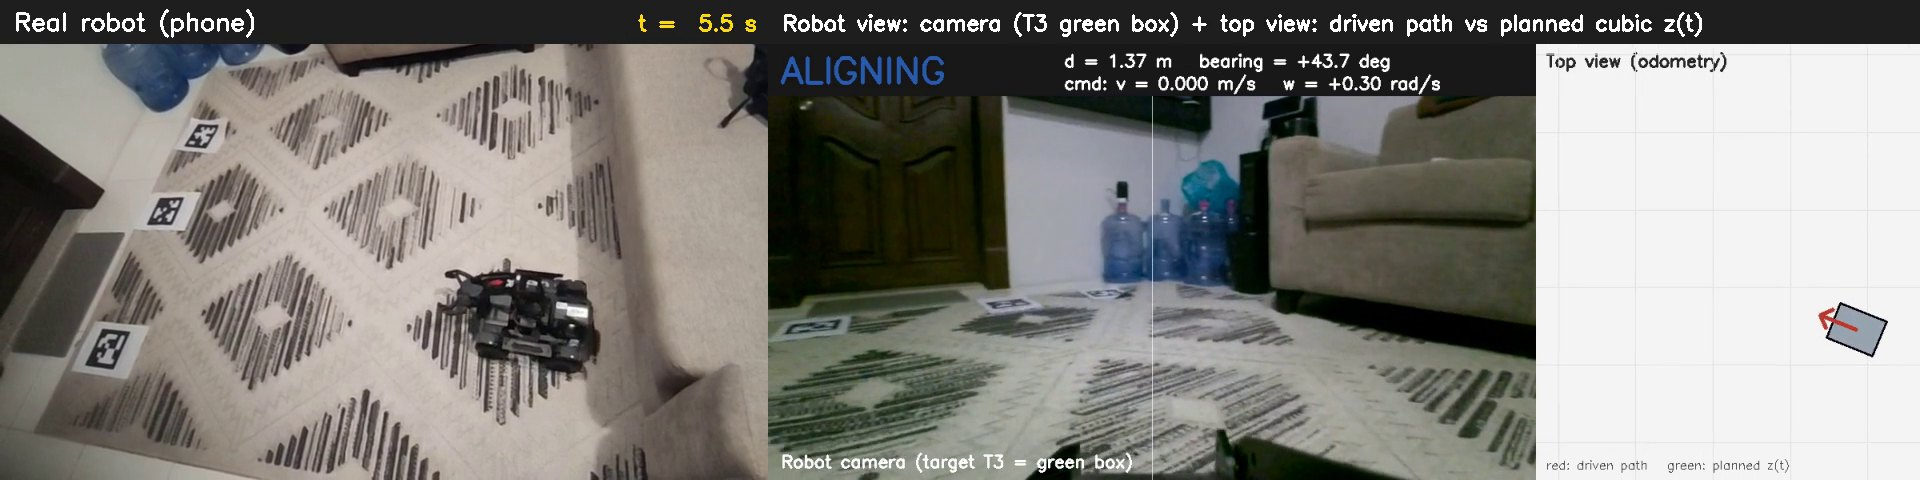
\includegraphics[width=\linewidth]{figures/still_aligning.jpg}
\caption{ALIGNING, $t=5.5$\,s: T3 just entered the camera image at $\theta=+43.7^\circ$, $d=1.37$\,m.}\end{subfigure}\\[3pt]
\begin{subfigure}{\linewidth}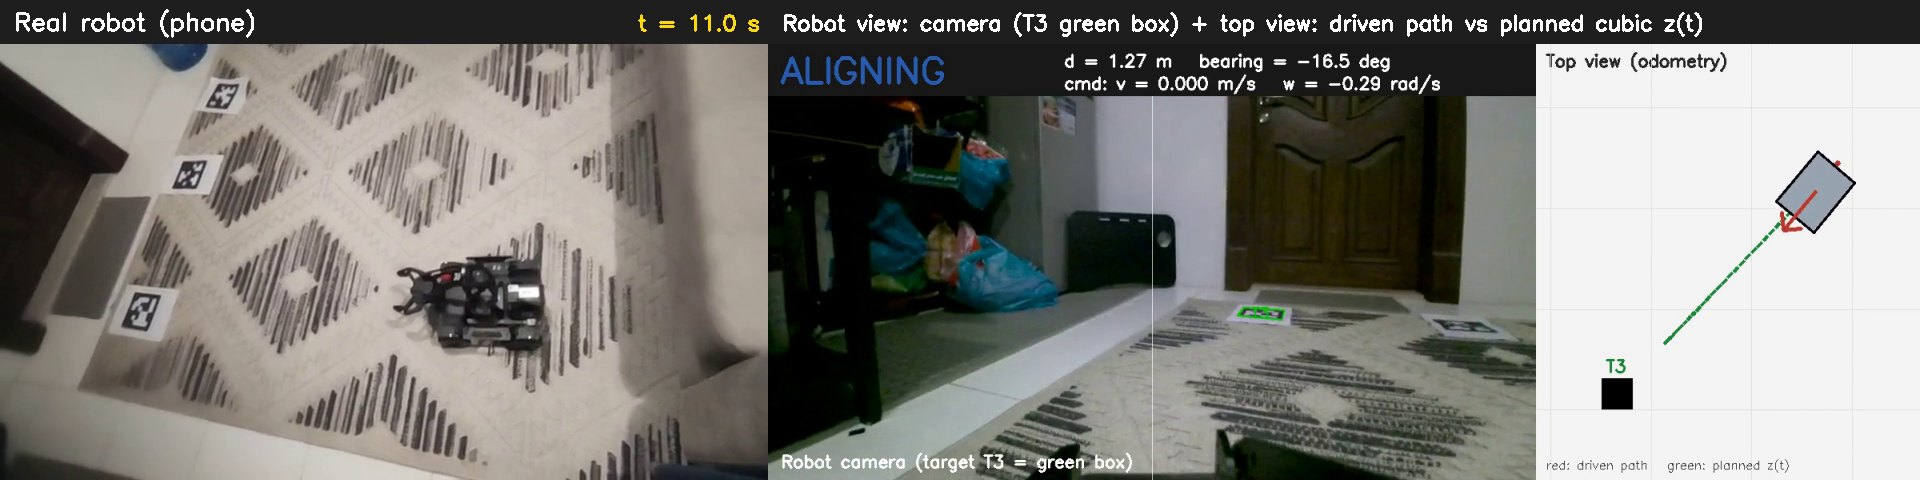
\includegraphics[width=\linewidth]{figures/still_realign.jpg}
\caption{ALIGNING again, $t=11.0$\,s: after the detection gap, T3 (green box) is centered with $\omega=-0.29$\,rad/s.}\end{subfigure}\\[3pt]
\begin{subfigure}{\linewidth}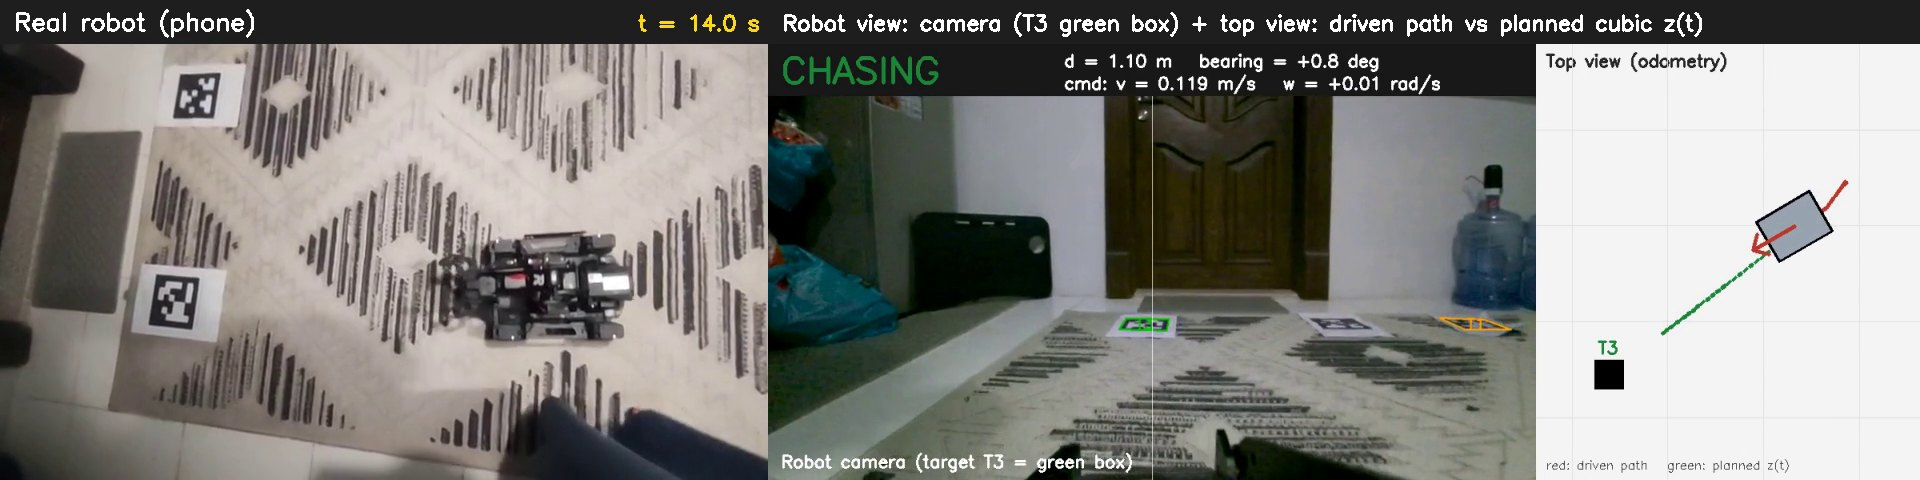
\includegraphics[width=\linewidth]{figures/still_chasing.jpg}
\caption{CHASING, $t=14.0$\,s: $d=1.10$\,m, $v=0.119$\,m/s along the cubic plan (green dots in the top view).}\end{subfigure}\\[3pt]
\begin{subfigure}{\linewidth}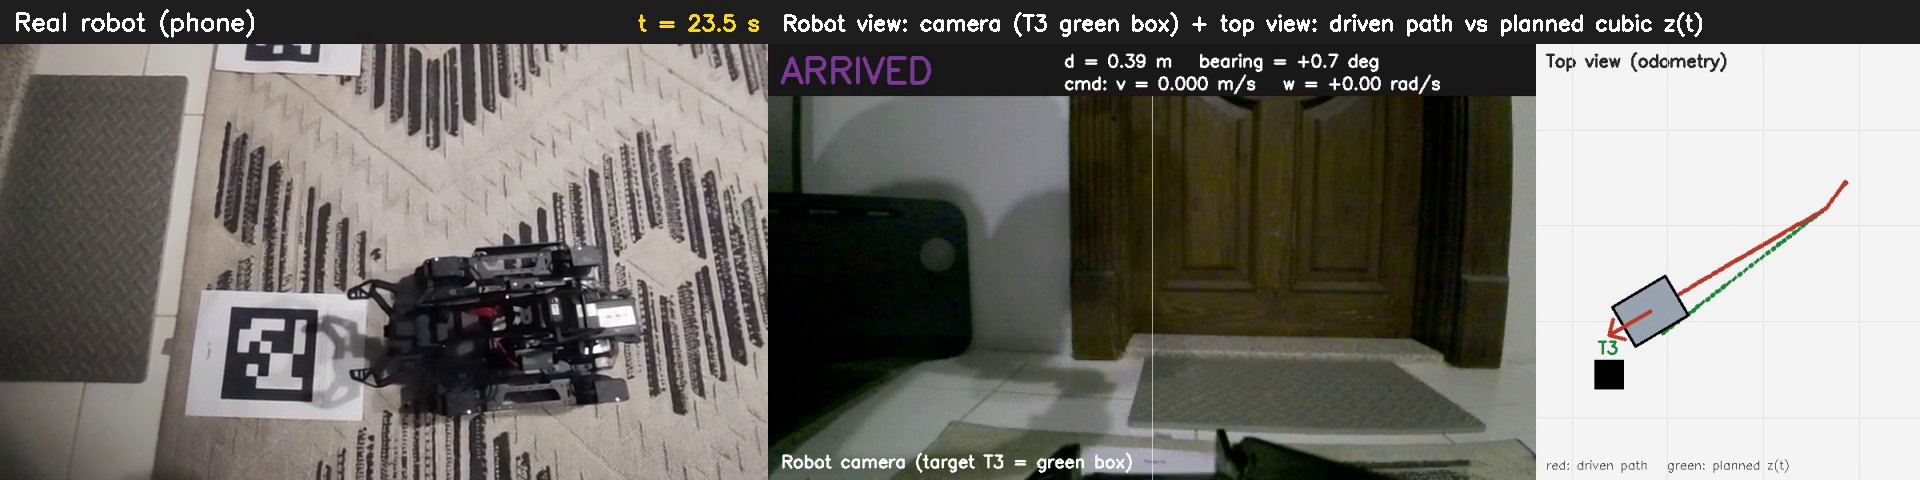
\includegraphics[width=\linewidth]{figures/still_arrived.jpg}
\caption{ARRIVED, $t=23.5$\,s: stopped 20\,cm before T3 (tape), command zero, all motor voltages 0.000\,V.}\end{subfigure}
\caption{Frames of the demonstration video (phone view, robot camera, top view).}
\label{fig:stills}
\end{figure}

%======================== 6. ENGINEERING ISSUES ================================
\isec{\faTools}{Engineering Issues and Lessons}

\isub{\faWifi}{Wi-Fi link: from direct AP to router mode}
\label{sec:wifi}
\begin{itemize}
  \item \textbf{Symptom:} in direct AP mode the laptop kept losing the robot (Table~\ref{tab:wifi}). The driver logs of the three AP sessions
        contain 23 \emph{Disconnected} events; in the longest session (27\,min) the link stayed up for a median of
        64.6\,s between drops (16 drops, 25 to 227\,s).
  \item \textbf{Cause on the host side:} the laptop's Realtek RTL8822CE card (driver \code{rtw_8822ce}) deauthenticated
        ``by local choice (Reason: 3=DEAUTH\_LEAVING)'', twelve times between 00:19:14 and 00:33:50, about 65\,s apart.
        Setting \code{disable_aspm=1} and \code{disable_lps_deep=1} for \code{rtw88} did not help: the next drop came
        60\,s after reconnecting (\code{notes/lab_log.md}).
  \item \textbf{Fix:} the robot was switched to router (STA) mode on the home 2.4\,GHz network, configured with a QR
        code generated by \code{tools/sta_qrcode.py} (the password is typed, never printed or saved). A 3\,min check
        (00:51:10 to 00:54:10) showed 0 deauth events, 0 driver disconnects and 0 detector re-subscribes with 10 to 15
        T3 detections/s (\code{notes/lab_log.md}); the driver log of the router-mode session then shows a single connection for 69\,min,
        covering all floor runs, until the session was ended after the final run.
  \item \textbf{Robustness kept in the code:} the detector re-subscribes to the camera after 2\,s without images, and
        the planner brakes if the tag is lost for more than 2\,s far from the goal.
\end{itemize}

\begin{table}[H]
\centering\small
\rowcolors{2}{kfupmlight}{white}
\begin{tabularx}{\linewidth}{@{}l c c c >{\raggedright\arraybackslash}X@{}}
\rowcolor{kfupm}\hd{Driver log} & \hd{Mode} & \hd{Span (min)} & \hd{Drops} & \hd{Connected time before a drop}\\
\code{driver_20261025_235452} & AP & 27.0 & 16 & median 64.6\,s, 25.0 to 227.2\,s\\
\code{driver_20261026_002315} & AP & 8.0 & 3 & median 130.1\,s, 64.1 to 263.2\,s\\
\code{driver_20261026_003846} & AP & 3.7 & 4 & median 41.1\,s, 14.0 to 64.1\,s\\
\code{driver_20261026_005040} & STA & 69.3 & 1 & one connection of 69\,min; the only drop came after the final run\\
\end{tabularx}
\caption{Connection events in the raw driver logs (\code{data/logs/}, parsed by \code{analysis/net_logs.py}).}
\label{tab:wifi}
\end{table}

\isub{\faWrench}{Other issues found on the robot}
Table~\ref{tab:issues} collects the remaining problems met during the assessment.
\begin{table}[H]
\centering\small
\rowcolors{2}{kfupmlight}{white}
\begin{tabularx}{\linewidth}{@{}>{\raggedright\arraybackslash}p{3.3cm}>{\raggedright\arraybackslash}X>{\raggedright\arraybackslash}X@{}}
\rowcolor{kfupm}\hd{Issue} & \hd{Evidence} & \hd{Resolution}\\
Arm pose hits the ToF sensor & arm hunts down to $z=0.050$\,m against the sensor (Section~\ref{sec:arm}, lab log) &
  arm set by hand 2\,cm above the sensor; planner arm guard ($\pm6$\,mm)\\
Driver $+x$ is away from the camera & 2\,s of $+0.05$\,m/s with wheels in the air: wheels turned away from the tag (lab log) & \code{drive_sign} $=-1$: \code{cmd_vel.linear.x} $=-v$; all
  logs stay in the mission frame\\
Arm TF wrong for this arm & TF gave $18^\circ$ and $22^\circ$ up; the floor tag gave $15.9^\circ$ down (lab log) & camera height and pitch from the
  floor tag (\code{extrinsics: tag})\\
Slant range at the standoff & 0.479\,m slant vs 0.362\,m ground (Figure~\ref{fig:geom}) & ground range in a level frame,
  offset within 6\,mm at 0.6 to 1.5\,m\\
Tag range limit & detected at 1.50\,m (3.8/s), ``NOT DETECTED in 8\,s'' at 1.80\,m (lab log) & runs start at 1.50\,m, the lower end of the specified
  range\\
Detection gaps at range & 4 restarts in run 1, 1.6\,s gap in run 2, 2.0\,s gap in the final run & chase tolerates gaps up
  to 2.0\,s; beyond that it searches again\\
Camera blind zone & no detection below 0.39\,m in any run & final approach on plan time and odometry\\
PyAV not installed & driver warning ``FFmpeg not available'' & raw images are enough; no change\\
Detector exit error & \code{RCLError} from a timer during shutdown, after the final run & harmless for the run; the
  planner, which owns \code{cmd_vel}, had already stopped\\
\end{tabularx}
\caption{Issues, the evidence for each, and how they were handled.}
\label{tab:issues}
\end{table}

\begin{keybox}{\faLightbulb\ \ Lessons learned}
\small
\begin{itemize}
  \item \textbf{Measure the frames on the robot itself.} Two conventions of the driver did not match this robot (drive
        direction and arm TF). A wheels-in-the-air test and one floor tag measured both directly.
  \item \textbf{A downward camera needs ground geometry.} Slant range overshoots the standoff by about 12\,cm here; the
        blind zone ends the visual feedback 0.19\,m before the stop.
  \item \textbf{Flatness makes the stop predictable.} Because the plan ends at $\dot x(T)=0$ exactly at $d_0-0.20$, the
        robot can finish the approach without the camera and still stop at 20\,cm.
  \item \textbf{Timeouts must match the sensor rate.} A 0.45\,s visibility rule suits searching, but a 4\,Hz detection
        stream at 1.5\,m needs a longer tolerance during the chase.
  \item \textbf{Fix the link before tuning the robot.} Most early failures were link drops, not control problems.
\end{itemize}
\end{keybox}

%============================= 7. CONCLUSIONS =================================
\isec{\faFlagCheckered}{Conclusions}
\begin{itemize}
  \item \textbf{Mission completed on the real robot.} In the filmed run the EP swept in place with T3 hidden, centered
        it, pursued it along a cubic flat-output plan and stopped 20\,cm before it (tape). The two earlier floor runs
        stopped at 21 and 20\,cm.
  \item \textbf{Flatness gives speed limits by construction.} With $T=\max(4,1.6(d_0-0.20)/v_{max})$ and
        $\dot x(0)=0.06$\,m/s the cubic peaks at 0.1371\,m/s for every $d_0>0.6$\,m; the measured command matched it.
  \item \textbf{Voltage telemetry behaves as the model predicts.} 0.456\,V in a steady search turn, about 1.06\,V at
        cruise, one-tick spikes at command steps, small negative voltages while braking and exactly 0.000\,V after the
        halt (Table~\ref{tab:table1}).
  \item \textbf{Two deviations, both documented.} The assignment arm pose collides with the ToF sensor on this robot, so
        a hand-set pose 2\,cm higher is used, guarded by the planner. At that pose the camera cannot see the tag at
        20\,cm, so the camera brake is implemented but the stops come from the plan and odometry.
  \item \textbf{Possible improvements:} a lower ToF mount that allows the assignment pose (steeper camera, camera
        brake active), a larger tag for the 1.8\,m end of the range, and measured wheel speeds from the ESCs to compare
        with the modeled voltages.
\end{itemize}

\begin{notebox}
\small\textbf{\color{kfupmdark}\faFolderOpen\ Reproducing the results} (after \code{source ~/rm_setup.sh})
\begin{itemize}
  \item Build: \code{cd ~/ros2_ws && colcon build --symlink-install --packages-select rm_flatness_nav}.
  \item Run: driver in its own terminal, then \code{ros2 launch rm_flatness_nav mission.launch.py}; the run folder with
        both CSV files is printed at start.
  \item Offline tests: \code{cd ros2/rm_flatness_nav && python3 -m pytest test} (36 tests).
  \item Figures, generated tables and \code{analysis/results/summary.md}: \code{python3 analysis/run_all.py}.
\end{itemize}
\end{notebox}

%============================== REFERENCES ====================================
\clearpage
\isec{\faBook}{References}
\begingroup\small
\renewcommand{\section}[2]{}%
\begin{thebibliography}{99}\setlength{\itemsep}{3pt}
\bibitem{assign} A.~I. Bhatti, \emph{SCE 672 Advanced Robotics, Term Project Assessment 2: Differential Flatness
  Pursuit and Motor Voltage Dynamics}, KFUPM, 2026.
\bibitem{lectures} A.~I. Bhatti, \emph{SCE 672 lecture notes}, Lectures 5A (actuators and wheel kinematics),
  5B (polynomial trajectories) and 6A (differential flatness), KFUPM, 2026.
\bibitem{fliess} M.~Fliess, J.~L\'evine, P.~Martin, and P.~Rouchon, ``Flatness and defect of non-linear systems:
  introductory theory and examples,'' \emph{International Journal of Control}, vol.~61, no.~6, pp.~1327-1361, 1995.
\bibitem{murray} R.~M. Murray, M.~Rathinam, and W.~Sluis, ``Differential flatness of mechanical control systems: a
  catalog of prototype systems,'' in \emph{Proc. ASME International Mechanical Engineering Congress and Exposition}, 1995.
\bibitem{lynch} K.~M. Lynch and F.~C. Park, \emph{Modern Robotics: Mechanics, Planning, and Control}. Cambridge
  University Press, 2017, Ch.~9 and~13.
\bibitem{siegwart} R.~Siegwart, I.~R. Nourbakhsh, and D.~Scaramuzza, \emph{Introduction to Autonomous Mobile Robots},
  2nd ed. MIT Press, 2011.
\bibitem{olson} E.~Olson, ``AprilTag: A robust and flexible visual fiducial system,'' in \emph{Proc. IEEE International
  Conference on Robotics and Automation (ICRA)}, 2011, pp.~3400-3407.
\bibitem{wang} J.~Wang and E.~Olson, ``AprilTag 2: Efficient and robust fiducial detection,'' in \emph{Proc. IEEE/RSJ
  International Conference on Intelligent Robots and Systems (IROS)}, 2016, pp.~4193-4198.
\bibitem{pupil} Pupil Labs, \emph{pupil-apriltags: Python bindings for the AprilTag library},
  \url{https://github.com/pupil-labs/apriltags}.
\bibitem{corke} P.~Corke, \emph{Robotics, Vision and Control}, 2nd ed. Springer, 2017.
\bibitem{rmros} J.~Guzzi, \emph{robomaster\_ros: ROS 2 driver for DJI RoboMaster EP and S1},
  \url{https://github.com/jeguzzi/robomaster_ros}.
\bibitem{djisdk} DJI, \emph{RoboMaster SDK Documentation}, \url{https://robomaster-dev.readthedocs.io}.
\bibitem{ros2} S.~Macenski, T.~Foote, B.~Gerkey, C.~Lalancette, and W.~Woodall, ``Robot Operating System 2: Design,
  architecture, and uses in the wild,'' \emph{Science Robotics}, vol.~7, no.~66, 2022.
\bibitem{rep103} T.~Foote and M.~Purvis, \emph{REP 103: Standard Units of Measure and Coordinate Conventions},
  \url{https://www.ros.org/reps/rep-0103.html}.
\end{thebibliography}
\endgroup

\begin{notebox}
\small\textbf{\color{kfupmdark}\faLightbulb\ Acknowledgement of AI assistance.}
I used Claude (Anthropic) as an assistant in this assessment, at my direction: it wrote the code (the ROS 2 package
\code{rm_flatness_nav}, the analysis scripts and the helper tools) and drafted this report, explaining each part so
that I can present and defend it. I performed all hardware setup, every robot run and every measurement (tape
standoffs, tag size, range calibration), recorded the videos, and reviewed the code, the results and the text against
the raw logs in the repository.
\end{notebox}


\end{document}
